\documentclass{article}
\usepackage[spanish]{babel}
\usepackage[utf8]{inputenc}
\usepackage[T1]{fontenc}
\usepackage{titlesec}
\usepackage{hyperref}
\usepackage{graphicx}
\usepackage{caption}
\usepackage{subcaption}
\usepackage{fancyhdr}
\usepackage[document]{ragged2e}
\pagestyle{fancy}
    \fancyhf{}
    \fancyfoot[C]{\thepage}
    \fancyfoot[L]{\ifodd\value{page}\textit{\small Gu\'ia de estudio Cl\'usters }\else\textit{\small Carlos E Martínez-Rodríguez}\fi}
    \fancyfoot[R]{\ifodd\value{page}\textit{\small Carlos E Martínez-Rodríguez}\else\textit{\small Gu\'ia de estudio Cl\'usters }\fi}
\usepackage[left=2cm,right=2cm,top=2cm,bottom=2cm]{geometry}
\renewcommand{\sectionmark}[1]{\markright{#1}}
\fancyhead[LE,RO]{\nouppercase{\rightmark}}
\fancyhead[LO,RE]{\nouppercase{\leftmark}}
% << == >>  << == >>  << == >>  << == >>  << == >>  << == >>  << == >>  << == >>  << == >>  << == >>  << == >> 
% Título y autor del documento
\title{An\'alisis de Cl\'usters, Componentes Principales y Mapas de Calor}
\author{Carlos E Martinez-Rodriguez}
% << == >>  << == >>  << == >>  << == >>  << == >>  << == >>  << == >>  << == >>  << == >>  << == >>  << == >> 
\begin{document}
% ============================================================================================================
\maketitle
\tableofcontents
\newpage
% ============================================================================================================
\section{Mapas de Calor}
% ============================================================================================================
\begin{itemize}
\item Introducción a los mapas de calor y su utilidad en la visualización de datos.
\item Construcción de mapas de calor utilizando diferentes técnicas y librerías, como Matplotlib, Seaborn, etc.
\item Personalización de los mapas de calor, incluyendo la selección de colores, escalas y anotaciones.
\item Interpretación de los mapas de calor y la identificación de patrones y tendencias en los datos.
\item Uso de mapas de calor en diferentes dominios, como análisis de expresión génica, análisis de datos climáticos, etc.

\end{itemize}

\subsection{Introducción}
Los mapas de calor son una herramienta visual poderosa utilizada en el análisis de datos para representar la distribución y la intensidad de una variable en una matriz de datos. Permiten identificar patrones, tendencias y anomalías de manera efectiva. En esta guía de estudio, exploraremos los conceptos básicos de los mapas de calor y su utilidad en la visualización de datos.

% <><> <><> <><> <><> <><> <><> <><> <><> <><> <><> <><> <><> <><> <><> <><> <><> <><> <><> <><> <><> <><> <><>
\subsection{Introducción a los mapas de calor}
% <><> <><> <><> <><> <><> <><> <><> <><> <><> <><> <><> <><> <><> <><> <><> <><> <><> <><> <><> <><> <><> <><>
Un mapa de calor es una representación gráfica en la que los valores de una matriz se muestran mediante colores. Cada celda de la matriz se asigna a un color según su valor, lo que permite visualizar fácilmente las variaciones en los datos. Los mapas de calor son especialmente útiles cuando se trabaja con matrices de datos grandes y multidimensionales.

% - - - - - - - -   - - - - - - - -   - - - - - - - -   - - - - - - - -   - - - - - - - - - - - - - - - - 
\subsubsection{Introducción}
Los mapas de calor son una herramienta visual ampliamente utilizada en el análisis de datos para representar la distribución y la intensidad de una variable en una matriz de datos. Permiten visualizar patrones, tendencias y variaciones en los datos de manera efectiva. En este documento, se proporcionará una introducción detallada a los mapas de calor y se explorará su utilidad en la visualización de datos.

% - - - - - - - -   - - - - - - - -   - - - - - - - -   - - - - - - - -   - - - - - - - - - - - - - - - - 
\subsubsection{Concepto de mapas de calor}
Un mapa de calor es una representación gráfica en la que los valores de una matriz se muestran mediante colores. Cada celda de la matriz se asigna a un color según su valor, lo que permite visualizar fácilmente las variaciones en los datos. Los mapas de calor se utilizan principalmente para mostrar la distribución espacial o temporal de una variable en un conjunto de datos.

% - - - - - - - -   - - - - - - - -   - - - - - - - -   - - - - - - - -   - - - - - - - - - - - - - - - - 
\subsubsection{Utilidad de los mapas de calor en la visualización de datos}
Los mapas de calor son especialmente útiles cuando se trabaja con conjuntos de datos grandes y multidimensionales. Algunas de las aplicaciones comunes de los mapas de calor en la visualización de datos incluyen:

\begin{itemize}
    \item Identificación de patrones y tendencias en datos climáticos y meteorológicos.
    \item Análisis de la distribución de la temperatura en imágenes térmicas.
    \item Visualización de datos de rendimiento en deportes para identificar fortalezas y debilidades.
    \item Análisis de expresión génica en biología molecular para identificar genes activos o inactivos.
    \item Representación de datos de mercado y finanzas para identificar áreas de crecimiento o declive.
\end{itemize}

% - - - - - - - -   - - - - - - - -   - - - - - - - -   - - - - - - - -   - - - - - - - - - - - - - - - - 
\subsubsection{Construcción de mapas de calor}
Existen varias técnicas y herramientas para construir mapas de calor. Algunas de las librerías y software populares utilizados incluyen Matplotlib, Seaborn, Tableau, entre otros. Estas herramientas proporcionan funciones y métodos para generar mapas de calor de manera eficiente y personalizable.

% - - - - - - - -   - - - - - - - -   - - - - - - - -   - - - - - - - -   - - - - - - - - - - - - - - - - 
\subsubsection{Personalización de los mapas de calor}
Los mapas de calor se pueden personalizar para adaptarse a las necesidades específicas de los datos y la visualización. Algunas de las opciones de personalización incluyen:

\begin{itemize}
    \item Selección de colores: es posible elegir una paleta de colores adecuada para resaltar las variaciones en los datos.
    \item Escalas de color: se pueden ajustar las escalas de color para resaltar áreas de alta o baja intensidad.
    \item Anotaciones y etiquetas: es posible agregar etiquetas y anotaciones a las celdas del mapa de calor para proporcionar información adicional.
\end{itemize}

% - - - - - - - -   - - - - - - - -   - - - - - - - -   - - - - - - - -   - - - - - - - - - - - - - - - - 
\subsubsection{Interpretación de los mapas de calor}
La interpretación de los mapas de calor es crucial para comprender la distribución de los datos. Algunos aspectos a considerar al interpretar los mapas de calor son:

\begin{itemize}
    \item Atención a la intensidad de los colores: los colores más intensos indican valores más altos o significativos, mientras que los colores más claros indican valores más bajos.
    \item Identificación de patrones y tendencias: buscar áreas de concentración o dispersión en el mapa de calor para identificar patrones y tendencias en los datos.
    \item Comparación entre mapas de calor: comparar diferentes mapas de calor para identificar diferencias o similitudes en la distribución de la variable en diferentes conjuntos de datos.
\end{itemize}

% - - - - - - - -   - - - - - - - -   - - - - - - - -   - - - - - - - -   - - - - - - - - - - - - - - - - 
\subsubsection*{Conclusiones}
En resumen, los mapas de calor son una valiosa herramienta en la visualización de datos, permitiendo identificar patrones, tendencias y variaciones en los datos de manera efectiva. Su construcción, personalización e interpretación adecuadas proporcionan una comprensión más profunda de los datos y facilitan la toma de decisiones basada en la información visualizada.


% <><> <><> <><> <><> <><> <><> <><> <><> <><> <><> <><> <><> <><> <><> <><> <><> <><> <><> <><> <><> <><> <><>
\subsection{Construcción de mapas de calor}
% <><> <><> <><> <><> <><> <><> <><> <><> <><> <><> <><> <><> <><> <><> <><> <><> <><> <><> <><> <><> <><> <><>

% - - - - - - - -   - - - - - - - -   - - - - - - - -   - - - - - - - -   - - - - - - - - - - - - - - - - 
\subsubsection{Introducción}
Los mapas de calor son una herramienta visual poderosa para visualizar la distribución de datos en forma de una matriz. R es un lenguaje de programación ampliamente utilizado en estadística y visualización de datos, y ofrece diversas librerías y funciones para construir mapas de calor de manera sencilla y efectiva. En este documento, se proporcionará una guía detallada sobre la construcción de mapas de calor en R.

% - - - - - - - -   - - - - - - - -   - - - - - - - -   - - - - - - - -   - - - - - - - - - - - - - - - - 
\subsubsection{Preparación de datos}
Antes de construir un mapa de calor en R, es importante preparar los datos adecuadamente. Asegúrate de tener una matriz o un dataframe con los datos que deseas visualizar. Asegúrate también de que los datos estén en el formato correcto y que no falten valores.

% - - - - - - - -   - - - - - - - -   - - - - - - - -   - - - - - - - -   - - - - - - - - - - - - - - - - 
\subsubsection{Librerías en R}
R ofrece varias librerías para construir mapas de calor. Algunas de las librerías más populares incluyen:

\begin{itemize}
    \item \textbf{heatmap}: Esta librería proporciona funciones para construir mapas de calor básicos en R.
    \item \textbf{ggplot2}: Esta librería, aunque principalmente utilizada para gráficos estadísticos, también ofrece funcionalidades para construir mapas de calor más avanzados y personalizables.
    \item \textbf{pheatmap}: Esta librería es una extensión de la librería heatmap y proporciona opciones adicionales para personalizar los mapas de calor.
\end{itemize}

% - - - - - - - -   - - - - - - - -   - - - - - - - -   - - - - - - - -   - - - - - - - - - - - - - - - - 
\subsubsection{Construcción de un mapa de calor básico con la librería heatmap}
A continuación se muestra un ejemplo de cómo construir un mapa de calor básico utilizando la librería heatmap en R:

\begin{verbatim}
# Cargar la librería heatmap
library(heatmap)

# Crear una matriz de ejemplo
matriz <- matrix(rnorm(100), nrow = 10)

# Construir el mapa de calor
heatmap(matriz)
\end{verbatim}

Este código generará un mapa de calor básico utilizando la función \texttt{heatmap} de la librería heatmap. Puedes ajustar los parámetros de la función según tus necesidades, como los colores utilizados, la escala, entre otros.

% - - - - - - - -   - - - - - - - -   - - - - - - - -   - - - - - - - -   - - - - - - - - - - - - - - - - 
\subsubsection{Construcción de un mapa de calor con la librería ggplot2}
Si deseas construir un mapa de calor más personalizable y estéticamente agradable, puedes utilizar la librería ggplot2. A continuación se muestra un ejemplo de cómo construir un mapa de calor utilizando la librería ggplot2:

\begin{verbatim}
# Cargar la librería ggplot2
library(ggplot2)

# Crear una matriz de ejemplo
matriz <- matrix(rnorm(100), nrow = 10)

# Convertir la matriz a un dataframe
df <- as.data.frame(matriz)

# Construir el mapa de calor utilizando ggplot2
ggplot(df, aes(x = factor(1), y = factor(1), fill = V1)) +
  geom_tile() +
  scale_fill_gradient(low = "blue", high = "red") +
  theme_void()
\end{verbatim}

Este código generará un mapa de calor utilizando la función \texttt{ggplot} de la librería ggplot2. Puedes personalizar el mapa de calor ajustando los parámetros de la función, como los colores utilizados, la escala, entre otros.

% - - - - - - - -   - - - - - - - -   - - - - - - - -   - - - - - - - -   - - - - - - - - - - - - - - - - 
\subsubsection*{Conclusiones}
En este documento se ha proporcionado una introducción a la construcción de mapas de calor en R. Se han presentado dos librerías populares, heatmap y ggplot2, y se ha mostrado cómo construir mapas de calor básicos utilizando estas librerías. Además, se ha destacado la importancia de la preparación adecuada de los datos antes de la construcción de los mapas de calor. 



% <><> <><> <><> <><> <><> <><> <><> <><> <><> <><> <><> <><> <><> <><> <><> <><> <><> <><> <><> <><> <><> <><>
\subsection{Personalización}
% <><> <><> <><> <><> <><> <><> <><> <><> <><> <><> <><> <><> <><> <><> <><> <><> <><> <><> <><> <><> <><> <><>


% - - - - - - - -   - - - - - - - -   - - - - - - - -   - - - - - - - -   - - - - - - - - - - - - - - - - 
\subsubsection{Introducción}
Los mapas de calor son una herramienta efectiva para visualizar datos en forma de una matriz. En R, existen varias librerías disponibles, como heatmap y ggplot2, que permiten construir mapas de calor. Además de la construcción básica de los mapas de calor, es posible personalizarlos según nuestras necesidades y preferencias. En este documento, se explorará la personalización de los mapas de calor en R, incluyendo la selección de colores, escalas y anotaciones.

% - - - - - - - -   - - - - - - - -   - - - - - - - -   - - - - - - - -   - - - - - - - - - - - - - - - - 
\subsubsection{Selección de colores}
La elección de colores es esencial para la interpretación adecuada de los mapas de calor. R ofrece varias paletas de colores predefinidas, pero también es posible definir colores personalizados. A continuación se muestra un ejemplo de cómo seleccionar colores para un mapa de calor en R:

\begin{verbatim}
# Cargar la librería heatmap
library(heatmap)

# Crear una matriz de ejemplo
matriz <- matrix(rnorm(100), nrow = 10)

# Definir una paleta de colores personalizada
mi_paleta <- colorRampPalette(c("blue", "white", "red"))

# Construir el mapa de calor utilizando la paleta de colores personalizada
heatmap(matriz, col = mi_paleta)
\end{verbatim}

En este ejemplo, se utiliza la función `colorRampPalette` para definir una paleta de colores que va desde el azul hasta el rojo. Esta paleta personalizada se pasa como argumento a la función `heatmap` para construir el mapa de calor.

% - - - - - - - -   - - - - - - - -   - - - - - - - -   - - - - - - - -   - - - - - - - - - - - - - - - - 
\subsubsection{Selección de escalas}
Además de los colores, es importante seleccionar la escala adecuada para los mapas de calor. R ofrece varias opciones de escalas, como escalas lineales y logarítmicas. A continuación se muestra un ejemplo de cómo seleccionar una escala para un mapa de calor en R:

\begin{verbatim}
# Cargar la librería pheatmap
library(pheatmap)

# Crear una matriz de ejemplo
matriz <- matrix(rnorm(100), nrow = 10)

# Construir el mapa de calor utilizando una escala logarítmica
pheatmap(matriz, scale = "log")
\end{verbatim}

En este ejemplo, se utiliza la función `pheatmap` de la librería pheatmap para construir el mapa de calor. El argumento `scale` se establece en "log" para utilizar una escala logarítmica en el mapa de calor.

% - - - - - - - -   - - - - - - - -   - - - - - - - -   - - - - - - - -   - - - - - - - - - - - - - - - - 
\subsubsection{Anotaciones en los mapas de calor}
Las anotaciones pueden proporcionar información adicional en los mapas de calor, como etiquetas de fila y columna, valores numéricos o etiquetas personalizadas. A continuación se muestra un ejemplo de cómo agregar anotaciones a un mapa de calor en R:

\begin{verbatim}
# Cargar la librería ComplexHeatmap
library(ComplexHeatmap)

# Crear una matriz de ejemplo
matriz <- matrix(rnorm(100), nrow = 10)

# Construir el mapa de calor con anotaciones de fila y columna
Heatmap(matriz, name = "Valor", row_names_side = "left", column_names_side = "top")
\end{verbatim}

En este ejemplo, se utiliza la función `Heatmap` de la librería ComplexHeatmap para construir el mapa de calor. Los argumentos `row\_names\_side` y `column\_names\_side` se establecen en "left" y "top", respectivamente, para agregar etiquetas de fila a la izquierda y etiquetas de columna en la parte superior del mapa de calor.

% - - - - - - - -   - - - - - - - -   - - - - - - - -   - - - - - - - -   - - - - - - - - - - - - - - - - 
\subsubsection*{Conclusiones}
En este documento, se ha explorado la personalización de los mapas de calor en R. Se ha mostrado cómo seleccionar colores personalizados, escalar los datos y agregar anotaciones para mejorar la interpretación de los mapas de calor. Recuerda que R ofrece una amplia variedad de librerías y funciones para la visualización de datos, por lo que puedes experimentar y adaptar estas técnicas según tus necesidades y preferencias.


% <><> <><> <><> <><> <><> <><> <><> <><> <><> <><> <><> <><> <><> <><> <><> <><> <><> <><> <><> <><> <><> <><>
\subsection{Interpretación de los mapas de calor }
% <><> <><> <><> <><> <><> <><> <><> <><> <><> <><> <><> <><> <><> <><> <><> <><> <><> <><> <><> <><> <><> <><>
% - - - - - - - -   - - - - - - - -   - - - - - - - -   - - - - - - - -   - - - - - - - - - - - - - - - - 
\subsubsection{Introducción}
Los mapas de calor son una herramienta poderosa para visualizar y explorar patrones y tendencias en conjuntos de datos. Permiten representar información en forma de una matriz coloreada, donde los colores representan los valores de los datos. En este documento, se explorará la interpretación de los mapas de calor y cómo identificar patrones y tendencias en los datos utilizando esta técnica.

% - - - - - - - -   - - - - - - - -   - - - - - - - -   - - - - - - - -   - - - - - - - - - - - - - - - - 
\subsubsection{Identificación de patrones}
Los mapas de calor son especialmente útiles para identificar patrones en los datos. Al observar un mapa de calor, se pueden identificar áreas de alta y baja intensidad, lo que puede indicar la presencia de patrones específicos. Algunas técnicas comunes para identificar patrones en los mapas de calor son:

\begin{itemize}
  \item \textbf{Patrones diagonales}: Los patrones diagonales en un mapa de calor pueden indicar una relación o correlación entre las variables representadas en los ejes.
  \item \textbf{Patrones repetitivos}: La repetición de ciertos colores o combinaciones de colores en diferentes secciones del mapa de calor puede indicar la presencia de patrones o estructuras repetitivas en los datos.
  \item \textbf{Patrones de gradiente}: Los patrones de cambio gradual en los colores de un mapa de calor pueden indicar una tendencia o una variación continua en los datos.
  \item \textbf{Agrupamiento de colores}: La agrupación de colores similares en áreas específicas del mapa de calor puede indicar la existencia de grupos o clusters en los datos.
\end{itemize}

Estas técnicas pueden ayudar a identificar patrones significativos en los datos y proporcionar información valiosa sobre las relaciones y estructuras presentes.

% - - - - - - - -   - - - - - - - -   - - - - - - - -   - - - - - - - -   - - - - - - - - - - - - - - - - 
\subsubsection{Identificación de tendencias}
Además de identificar patrones, los mapas de calor también pueden revelar tendencias en los datos. Al observar la distribución de colores en un mapa de calor, se pueden identificar tendencias ascendentes o descendentes en los valores de los datos. Algunos enfoques comunes para identificar tendencias en los mapas de calor son:

\begin{itemize}
  \item \textbf{Tendencias verticales}: Las tendencias verticales en un mapa de calor pueden indicar cambios sistemáticos en los datos a medida que se mueven a lo largo del eje vertical. Estas tendencias pueden sugerir patrones de tiempo o alguna otra dimensión específica.
  \item \textbf{Tendencias horizontales}: Las tendencias horizontales en un mapa de calor pueden indicar cambios sistemáticos en los datos a medida que se mueven a lo largo del eje horizontal. Estas tendencias pueden indicar variaciones en otras dimensiones o variables.
  \item \textbf{Tendencias diagonales}: Las tendencias diagonales en un mapa de calor pueden revelar relaciones o correlaciones entre las variables representadas en los ejes, lo que indica cambios conjuntos en los datos.
  \item \textbf{Tendencias globales}: Las tendencias globales se refieren a los cambios generales o dominantes que se pueden observar en todo el mapa de calor. Estas tendencias pueden indicar características importantes de los datos.
\end{itemize}

La identificación de tendencias en los mapas de calor puede ayudar a comprender mejor los datos y proporcionar información útil para análisis posteriores.

% - - - - - - - -   - - - - - - - -   - - - - - - - -   - - - - - - - -   - - - - - - - - - - - - - - - - 
\subsubsection{Ejemplo de interpretación}
Para ilustrar la interpretación de los mapas de calor, se presenta un ejemplo utilizando un conjunto de datos de temperaturas mensuales promedio en diferentes regiones geográficas. La Figura \ref{fig:heatmap_example} muestra un mapa de calor que representa estos datos.

\begin{figure}[htbp]
  \centering
  \includegraphics[width=0.8\textwidth]{MapadeCalorFinalCorregido.pdf}
  \caption{Ejemplo de mapa de calor de temperaturas mensuales promedio en diferentes regiones geográficas.}
  \label{fig:heatmap_example}
\end{figure}

Al analizar este mapa de calor, se pueden realizar las siguientes observaciones:

\begin{itemize}
  \item Hay una clara tendencia ascendente de colores más claros (temperaturas más bajas) en la parte superior del mapa de calor a colores más oscuros (temperaturas más altas) en la parte inferior. Esto indica una tendencia de aumento de temperatura de norte a sur.
  \item Se pueden observar patrones diagonales en varias regiones, lo que sugiere una correlación entre las temperaturas de diferentes regiones geográficas.
  \item Hay áreas específicas con colores más oscuros o más claros, lo que indica la presencia de patrones locales o regionales de temperaturas más altas o más bajas.
\end{itemize}

Estas observaciones nos proporcionan información valiosa sobre las tendencias y patrones presentes en los datos de temperaturas mensuales promedio.

% - - - - - - - -   - - - - - - - -   - - - - - - - -   - - - - - - - -   - - - - - - - - - - - - - - - - 
\subsubsection*{Conclusiones}
En este documento, se ha explorado la interpretación de los mapas de calor y la identificación de patrones y tendencias en los datos. Se han presentado técnicas y enfoques para identificar patrones y tendencias en los mapas de calor, y se ha proporcionado un ejemplo ilustrativo. Los mapas de calor son una herramienta poderosa en la visualización de datos, y su interpretación adecuada puede revelar información valiosa para el análisis y la toma de decisiones.



% <><> <><> <><> <><> <><> <><> <><> <><> <><> <><> <><> <><> <><> <><> <><> <><> <><> <><> <><> <><> <><> <><>
\subsection{Uso de mapas de calor}
% <><> <><> <><> <><> <><> <><> <><> <><> <><> <><> <><> <><> <><> <><> <><> <><> <><> <><> <><> <><> <><> <><>



% - - - - - - - -   - - - - - - - -   - - - - - - - -   - - - - - - - -   - - - - - - - - - - - - - - - - 
\subsubsection{Introducción}
Los mapas de calor son una herramienta versátil de visualización de datos que se pueden aplicar en diversos dominios. En este documento, exploraremos el uso de mapas de calor en diferentes áreas, como el análisis de expresión génica, el análisis de datos climáticos y otros campos relacionados.

% - - - - - - - -   - - - - - - - -   - - - - - - - -   - - - - - - - -   - - - - - - - - - - - - - - - - 
\subsubsection{Análisis de expresión génica}
El análisis de expresión génica es un campo importante en la genómica, donde se investiga la actividad de los genes en diferentes condiciones. Los mapas de calor son ampliamente utilizados para visualizar los perfiles de expresión génica. En este contexto, cada fila del mapa de calor representa un gen, y cada columna representa una muestra o condición. Los valores de expresión se representan mediante colores, lo que permite identificar patrones de expresión diferencial y agrupamientos de genes con perfiles similares.

% - - - - - - - -   - - - - - - - -   - - - - - - - -   - - - - - - - -   - - - - - - - - - - - - - - - - 
\subsubsection{Análisis de datos climáticos}
En el análisis de datos climáticos, los mapas de calor son utilizados para visualizar y comprender las variaciones espaciales y temporales de las variables climáticas. Por ejemplo, se pueden crear mapas de calor para mostrar la distribución de temperaturas, precipitaciones o niveles de contaminantes en diferentes regiones. Esto ayuda a identificar patrones climáticos, como áreas de altas temperaturas o regiones con altos niveles de precipitación.

% - - - - - - - -   - - - - - - - -   - - - - - - - -   - - - - - - - -   - - - - - - - - - - - - - - - - 
\subsubsection{Análisis de datos financieros}
En el análisis financiero, los mapas de calor son útiles para visualizar y analizar la correlación entre diferentes activos financieros. Por ejemplo, se pueden utilizar mapas de calor para mostrar la matriz de correlación entre los precios de diferentes acciones. Esto permite identificar relaciones positivas o negativas entre los activos y detectar patrones de agrupamiento o diversificación en una cartera de inversiones.

% - - - - - - - -   - - - - - - - -   - - - - - - - -   - - - - - - - -   - - - - - - - - - - - - - - - - 
\subsubsection{Análisis de datos de redes sociales}
En el análisis de datos de redes sociales, los mapas de calor son utilizados para visualizar patrones de interacción entre usuarios. Por ejemplo, se pueden construir mapas de calor para mostrar la frecuencia de interacción entre diferentes usuarios en una plataforma de redes sociales. Esto puede revelar comunidades o grupos de usuarios que interactúan con mayor frecuencia y detectar nodos clave dentro de la red social.

% - - - - - - - -   - - - - - - - -   - - - - - - - -   - - - - - - - -   - - - - - - - - - - - - - - - - 
\subsubsection*{Conclusiones}
Los mapas de calor son una herramienta poderosa para visualizar y analizar datos en diferentes dominios. Se pueden aplicar en áreas como el análisis de expresión génica, el análisis de datos climáticos, el análisis financiero y el análisis de datos de redes sociales, entre otros. La capacidad de identificar patrones y tendencias en los datos mediante mapas de calor proporciona información valiosa para la toma de decisiones y el descubrimiento de conocimiento en diferentes campos.

Es importante tener en cuenta que el uso adecuado de los mapas de calor requiere una comprensión profunda del dominio de aplicación y una interpretación cuidadosa de los resultados. Además, la elección de colores, escalas y anotaciones adecuadas es fundamental para garantizar una representación clara y precisa de los datos.




\newpage
% ============================================================================================================
\section{Introducción al an\'alisis de cl\'usters}
% ============================================================================================================
\begin{itemize}
\item Introducción al análisis de clusters y su importancia en la minería de datos y la estadística.
\item Tipos de algoritmos de clustering, como k-means, agrupamiento jerárquico, DBSCAN, etc.
\item Métricas de evaluación de clusters, como el coeficiente de silueta, índices de calidad interna y externa, etc.
\item Preprocesamiento de datos para el análisis de clusters, incluyendo la normalización y la selección de características.
\item Técnicas avanzadas de clustering, como el clustering espectral, el clustering basado en densidad, etc.
\item Aplicaciones del análisis de clusters en diferentes áreas, como marketing, bioinformática, reconocimiento de patrones, etc.
\end{itemize}

% <><> <><> <><> <><> <><> <><> <><> <><> <><> <><> <><> <><> <><> <><> <><> <><> <><> <><> <><> <><> <><> <><>
\subsection{Análisis de Clusters}
% <><> <><> <><> <><> <><> <><> <><> <><> <><> <><> <><> <><> <><> <><> <><> <><> <><> <><> <><> <><> <><> <><>

%    - - - - - - - -   - - - - - - - -   - - - - - - - -   - - - - - - - -   - - - - - - - - - - - - - - - - 
\subsubsection{An\'alisis de cl\'usters}
%    - - - - - - - -   - - - - - - - -   - - - - - - - -   - - - - - - - -   - - - - - - - - - - - - - - - - 

El análisis de clusters es una técnica fundamental en la minería de datos y la estadística que permite identificar grupos o clusters dentro de conjuntos de datos. Estos grupos se forman en base a similitudes o patrones encontrados en las características de los datos, lo que facilita la comprensión y exploración de la estructura subyacente de los mismos.

En este documento, se presentará una introducción al análisis de clusters, explicando sus conceptos básicos, aplicaciones en la minería de datos y la estadística, así como los diferentes enfoques y algoritmos utilizados para llevar a cabo este análisis.
%    - - - - - - - -   - - - - - - - -   - - - - - - - -   - - - - - - - -   - - - - - - - - - - - - - - - - 
\subsubsection{Conceptos básicos del análisis de clusters}
%    - - - - - - - -   - - - - - - - -   - - - - - - - -   - - - - - - - -   - - - - - - - - - - - - - - - - 
El análisis de clusters se basa en la idea de que los datos pueden agruparse en conjuntos o clusters, donde los objetos dentro de un mismo cluster son más similares entre sí que con los objetos de otros clusters. Para entender este concepto, es importante familiarizarse con los siguientes términos:

\begin{itemize}
  \item \textbf{Objeto o elemento}: Es una entidad individual que se analiza y se agrupa en clusters.
  \item \textbf{Característica}: Es una medida o atributo que se utiliza para describir un objeto.
  \item \textbf{Similitud o distancia}: Es una medida que indica qué tan parecidos o diferentes son dos objetos en función de sus características. Puede calcularse utilizando diversas métricas, como la distancia euclidiana o la distancia de Manhattan.
  \item \textbf{Centroide}: Es un punto representativo dentro de un cluster que resume las características de los objetos en ese grupo.
\end{itemize}
%    - - - - - - - -   - - - - - - - -   - - - - - - - -   - - - - - - - -   - - - - - - - - - - - - - - - - 
\subsubsection{Aplicaciones del análisis de clusters}
%    - - - - - - - -   - - - - - - - -   - - - - - - - -   - - - - - - - -   - - - - - - - - - - - - - - - - 
El análisis de clusters tiene numerosas aplicaciones en diferentes áreas, incluyendo la minería de datos y la estadística. Algunas de las aplicaciones más comunes son:

\begin{itemize}
  \item Segmentación de clientes: Permite identificar grupos de clientes con características similares, lo que ayuda a personalizar estrategias de marketing y ofrecer productos o servicios adaptados a cada segmento.
  \item Análisis de mercado: Permite identificar grupos de productos o áreas geográficas con comportamientos similares, lo que facilita la toma de decisiones estratégicas en términos de precios, distribución y promoción.
  \item Análisis de genes: Permite identificar grupos de genes con expresiones similares, lo que ayuda a comprender la función y relación entre ellos en el contexto de la genética y la biología.
  \item Análisis de texto: Permite agrupar documentos o textos similares en función de su contenido, lo que facilita la organización y clasificación de grandes volúmenes de información.
\end{itemize}
%    - - - - - - - -   - - - - - - - -   - - - - - - - -   - - - - - - - -   - - - - - - - - - - - - - - - - 
\subsubsection{Enfoques y algoritmos de análisis de clusters}
%    - - - - - - - -   - - - - - - - -   - - - - - - - -   - - - - - - - -   - - - - - - - - - - - - - - - - 
Existen diferentes enfoques y algoritmos para realizar el análisis de clusters, dependiendo de las características de los datos y los objetivos del estudio. Algunos de los enfoques más utilizados son:

\begin{itemize}
  \item \textbf{Clustering jerárquico}: Agrupa los objetos en forma de un árbol jerárquico, donde los clusters se fusionan o dividen en función de la similitud entre ellos. Puede ser aglomerativo (de abajo hacia arriba) o divisivo (de arriba hacia abajo).
  \item \textbf{Clustering particional}: Asigna cada objeto a un cluster en base a ciertos criterios, como minimizar la distancia entre los objetos dentro de un cluster y maximizar la distancia entre los objetos de diferentes clusters. Ejemplos de algoritmos particionales son k-means y k-medoids.
  \item \textbf{Clustering basado en densidad}: Identifica áreas densas de objetos en el espacio de características y separa regiones menos densas. El algoritmo DBSCAN es un ejemplo popular de clustering basado en densidad.
\end{itemize}
%    - - - - - - - -   - - - - - - - -   - - - - - - - -   - - - - - - - -   - - - - - - - - - - - - - - - - 
\subsubsection*{Conclusiones}
%    - - - - - - - -   - - - - - - - -   - - - - - - - -   - - - - - - - -   - - - - - - - - - - - - - - - - 
El análisis de clusters es una técnica poderosa para descubrir patrones y estructuras en conjuntos de datos, lo que lo convierte en una herramienta esencial en la minería de datos y la estadística. Permite agrupar objetos similares, lo que facilita la comprensión y el análisis de grandes volúmenes de información.
% <><> <><> <><> <><> <><> <><> <><> <><> <><> <><> <><> <><> <><> <><> <><> <><> <><> <><> <><> <><> <><> <><>
\subsection{Tipos de algoritmos de clustering}
% <><> <><> <><> <><> <><> <><> <><> <><> <><> <><> <><> <><> <><> <><> <><> <><> <><> <><> <><> <><> <><> <><>
%    - - - - - - - -   - - - - - - - -   - - - - - - - -   - - - - - - - -   - - - - - - - - - - - - - - - - 
\subsubsection{Introducción}
%    - - - - - - - -   - - - - - - - -   - - - - - - - -   - - - - - - - -   - - - - - - - - - - - - - - - - 
El clustering es una técnica fundamental en la minería de datos y la estadística que permite agrupar objetos similares en conjuntos o clusters. Existen varios tipos de algoritmos de clustering, cada uno con sus propias características y aplicaciones. En este documento, se presentarán algunos de los tipos más comunes, como k-means, agrupamiento jerárquico y DBSCAN, y se explicará su funcionamiento y ventajas.
%    - - - - - - - -   - - - - - - - -   - - - - - - - -   - - - - - - - -   - - - - - - - - - - - - - - - - 
\subsubsection{K-means}
%    - - - - - - - -   - - - - - - - -   - - - - - - - -   - - - - - - - -   - - - - - - - - - - - - - - - - 
El algoritmo de k-means es uno de los métodos de clustering más utilizados. El objetivo de este algoritmo es particionar un conjunto de datos en k clusters, donde k es un número predefinido. El algoritmo funciona de la siguiente manera:

\begin{enumerate}
  \item Seleccionar k centroides iniciales de forma aleatoria o utilizando algún criterio específico.
  \item Asignar cada objeto al centroide más cercano.
  \item Recalcular los centroides como la media de los objetos asignados a cada cluster.
  \item Repetir los pasos 2 y 3 hasta que no haya cambios en las asignaciones de los objetos o se alcance un criterio de convergencia.
\end{enumerate}

El algoritmo de k-means tiene la ventaja de ser eficiente y fácil de implementar. Sin embargo, tiene algunas limitaciones, como la sensibilidad a la inicialización de los centroides y la asunción de que los clusters tienen formas esféricas y tamaños similares.
%    - - - - - - - -   - - - - - - - -   - - - - - - - -   - - - - - - - -   - - - - - - - - - - - - - - - - 
\subsubsection{Agrupamiento jerárquico}
%    - - - - - - - -   - - - - - - - -   - - - - - - - -   - - - - - - - -   - - - - - - - - - - - - - - - - 
El agrupamiento jerárquico es otro enfoque popular en el análisis de clustering. Este tipo de algoritmo construye una estructura jerárquica de clusters, donde los clusters se agrupan o dividen en base a la similitud entre ellos. Hay dos tipos de agrupamiento jerárquico:

\begin{itemize}
  \item \textbf{Aglomerativo}: Comienza con cada objeto como un cluster individual y fusiona los clusters más cercanos en cada paso hasta obtener un único cluster que contiene todos los objetos.
  \item \textbf{Divisivo}: Comienza con un único cluster que contiene todos los objetos y divide los clusters existentes en cada paso hasta obtener clusters individuales para cada objeto.
\end{itemize}

El agrupamiento jerárquico tiene la ventaja de proporcionar una visión estructurada y completa de los datos, permitiendo explorar diferentes niveles de granularidad en los clusters. Sin embargo, puede ser computacionalmente costoso en conjuntos de datos grandes.
%    - - - - - - - -   - - - - - - - -   - - - - - - - -   - - - - - - - -   - - - - - - - - - - - - - - - - 
\subsubsection{DBSCAN}
%    - - - - - - - -   - - - - - - - -   - - - - - - - -   - - - - - - - -   - - - - - - - - - - - - - - - - 
DBSCAN (Density-Based Spatial Clustering of Applications with Noise) es un algoritmo de clustering basado en densidad. A diferencia de k-means y el agrupamiento jerárquico, DBSCAN no requiere especificar el número de clusters de antemano. En su lugar, identifica áreas densas de objetos en el espacio de características y separa regiones menos densas. El algoritmo funciona de la siguiente manera:

\begin{enumerate}
  \item Seleccionar un objeto no visitado aleatoriamente.
  \item Si el objeto tiene suficientes vecinos cercanos, se forma un nuevo cluster a partir de él y sus vecinos. Se marcan los objetos visitados.
  \item Se repite el proceso para los vecinos del nuevo cluster hasta que no se encuentren más objetos visitables.
  \item Si aún quedan objetos no visitados, se selecciona otro objeto y se repite el proceso.
\end{enumerate}

DBSCAN es capaz de encontrar clusters de cualquier forma y tamaño, y puede identificar puntos de ruido o valores atípicos. Sin embargo, puede tener dificultades en conjuntos de datos de alta dimensionalidad.
%    - - - - - - - -   - - - - - - - -   - - - - - - - -   - - - - - - - -   - - - - - - - - - - - - - - - - 
\subsubsection*{Conclusiones}
%    - - - - - - - -   - - - - - - - -   - - - - - - - -   - - - - - - - -   - - - - - - - - - - - - - - - - 
En este documento, se han presentado algunos de los tipos de algoritmos de clustering más comunes, como k-means, agrupamiento jerárquico y DBSCAN. Cada tipo de algoritmo tiene sus propias características, ventajas y limitaciones, por lo que es importante seleccionar el algoritmo adecuado según las características del conjunto de datos y los objetivos del análisis.

% <><> <><> <><> <><> <><> <><> <><> <><> <><> <><> <><> <><> <><> <><> <><> <><> <><> <><> <><> <><> <><> <><>
\subsection{Métricas de Evaluación de Clusters}
% <><> <><> <><> <><> <><> <><> <><> <><> <><> <><> <><> <><> <><> <><> <><> <><> <><> <><> <><> <><> <><> <><>

%    - - - - - - - -   - - - - - - - -   - - - - - - - -   - - - - - - - -   - - - - - - - - - - - - - - - - 
\subsubsection{Introducción}
En esta sección, proporciona una introducción al tema de las métricas de evaluación de clusters. Explica la importancia de evaluar la calidad de los clusters obtenidos en un análisis de clustering y cómo las métricas de evaluación pueden ayudar en este proceso.

%    - - - - - - - -   - - - - - - - -   - - - - - - - -   - - - - - - - -   - - - - - - - - - - - - - - - - 
\subsubsection{Coeficiente de Silueta}
En esta sección, describe en detalle el coeficiente de silueta como una métrica de evaluación comúnmente utilizada en clustering. Explica cómo se calcula el coeficiente de silueta y cómo se interpreta. Menciona las ventajas y limitaciones de esta métrica y proporciona ejemplos de su uso en casos prácticos.

%    - - - - - - - -   - - - - - - - -   - - - - - - - -   - - - - - - - -   - - - - - - - - - - - - - - - - 
\subsubsection{Índices de Calidad Interna}
En esta sección, discute los índices de calidad interna como métricas de evaluación de clusters. Presenta diferentes índices, como el índice de Davies-Bouldin, el índice de Calinski-Harabasz y el índice de Dunn. Explica cómo se calculan y cómo se interpretan. Discute las ventajas y limitaciones de cada índice y proporciona ejemplos de su aplicación.

%    - - - - - - - -   - - - - - - - -   - - - - - - - -   - - - - - - - -   - - - - - - - - - - - - - - - - 
\subsubsection{Índices de Calidad Externa}
En esta sección, explora los índices de calidad externa como métricas de evaluación de clusters que utilizan información externa, como etiquetas o clases conocidas. Presenta índices como el índice de Rand ajustado y el índice de Fowlkes-Mallows. Explica cómo se calculan y cómo se interpretan. Discute las ventajas y limitaciones de estos índices y proporciona ejemplos de su uso en evaluaciones externas de clusters.

%    - - - - - - - -   - - - - - - - -   - - - - - - - -   - - - - - - - -   - - - - - - - - - - - - - - - - 
\subsubsection{Otras Métricas de Evaluación}
En esta sección, menciona otras métricas de evaluación de clusters que pueden ser relevantes según el contexto específico. Esto puede incluir métricas para la detección de outliers, métricas para clusters con estructuras específicas, etc. Proporciona ejemplos y discute las aplicaciones de estas métricas.

%    - - - - - - - -   - - - - - - - -   - - - - - - - -   - - - - - - - -   - - - - - - - - - - - - - - - - 
\subsubsection*{Conclusiones}
En esta sección, resume las principales métricas de evaluación de clusters discutidas en el documento. Destaca la importancia de evaluar la calidad de los clusters y el papel fundamental que desempeñan estas métricas en el análisis de clustering. Menciona las ventajas y limitaciones de cada métrica y sugiere posibles áreas de investigación futura.

% <><> <><> <><> <><> <><> <><> <><> <><> <><> <><> <><> <><> <><> <><> <><> <><> <><> <><> <><> <><> <><> <><>
\subsection{Preprocesamiento de datos}
% <><> <><> <><> <><> <><> <><> <><> <><> <><> <><> <><> <><> <><> <><> <><> <><> <><> <><> <><> <><> <><> <><>

%    - - - - - - - -   - - - - - - - -   - - - - - - - -   - - - - - - - -   - - - - - - - - - - - - - - - - 
\subsubsection{Introducción}
En el campo del análisis de datos, el análisis de clusters juega un papel fundamental para descubrir patrones y estructuras ocultas en conjuntos de datos. Sin embargo, antes de aplicar cualquier algoritmo de clustering, es crucial realizar un adecuado preprocesamiento de los datos. El preprocesamiento incluye una serie de técnicas que permiten preparar los datos para su posterior análisis, y entre ellas se destacan la normalización y la selección de características. Este documento se centra en explorar estas dos técnicas y su importancia en el análisis de clusters.

%    - - - - - - - -   - - - - - - - -   - - - - - - - -   - - - - - - - -   - - - - - - - - - - - - - - - - 
\subsubsection{Normalización de datos}
La normalización de datos es un paso esencial en el preprocesamiento de datos antes de aplicar técnicas de clustering. El objetivo de la normalización es llevar los datos a una escala común y eliminar cualquier sesgo causado por diferencias en las unidades o magnitudes de las variables. En esta sección se presentan algunas de las técnicas de normalización más utilizadas, como la normalización min-max, la estandarización y la normalización por escala logarítmica.

%    - - - - - - - -   - - - - - - - -   - - - - - - - -   - - - - - - - -   - - - - - - - - - - - - - - - - 
\subsubsection{Normalización min-max}
La normalización min-max es un método común para escalar los datos en un rango específico, generalmente entre 0 y 1. Consiste en restar el valor mínimo de cada variable y luego dividir por la diferencia entre el valor máximo y el valor mínimo. Esta técnica garantiza que todos los valores estén dentro del rango deseado, preservando las proporciones relativas entre ellos.

%    - - - - - - - -   - - - - - - - -   - - - - - - - -   - - - - - - - -   - - - - - - - - - - - - - - - - 
\subsubsection{Estandarización}
La estandarización, también conocida como z-score normalization, transforma los datos de manera que tengan una media de 0 y una desviación estándar de 1. Esto se logra restando la media de cada variable y dividiendo por la desviación estándar. La estandarización es útil cuando las variables tienen diferentes unidades o varían en escalas diferentes.

%    - - - - - - - -   - - - - - - - -   - - - - - - - -   - - - - - - - -   - - - - - - - - - - - - - - - - 
\subsubsection{Normalización por escala logarítmica}
En algunos casos, los datos pueden tener una distribución asimétrica o con valores extremadamente grandes o pequeños. En estas situaciones, la normalización por escala logarítmica puede ser beneficiosa. Consiste en aplicar el logaritmo a los datos, lo que reduce la varianza de los valores extremos y los acerca a una distribución más simétrica.

%    - - - - - - - -   - - - - - - - -   - - - - - - - -   - - - - - - - -   - - - - - - - - - - - - - - - - 
\subsubsection{Selección de características}
La selección de características es otro paso importante en el preprocesamiento de datos antes del análisis de clusters. El objetivo de esta técnica es identificar y seleccionar las variables más relevantes o representativas que contribuyen significativamente al proceso de clustering. En esta sección se presentan diferentes métodos de selección de características, como la selección basada en filtros, la selección basada en wrappers y la selección basada en incrustación.

%    - - - - - - - -   - - - - - - - -   - - - - - - - -   - - - - - - - -   - - - - - - - - - - - - - - - - 
\subsubsection{Selección basada en filtros}
La selección basada en filtros se basa en el análisis de la correlación o la importancia estadística de las variables. Se calculan métricas de relevancia para cada variable y se seleccionan las mejores según un umbral predefinido. Algunas de las métricas comunes incluyen la correlación de Pearson, la ganancia de información y la prueba F.

%    - - - - - - - -   - - - - - - - -   - - - - - - - -   - - - - - - - -   - - - - - - - - - - - - - - - - 
\subsubsection{Selección basada en wrappers}
La selección basada en wrappers involucra la evaluación de los algoritmos de clustering utilizando diferentes subconjuntos de variables. Se utilizan técnicas de búsqueda exhaustiva o heurísticas para encontrar la combinación óptima de variables que maximice un criterio de evaluación específico, como la precisión de clustering. Sin embargo, este enfoque puede ser computacionalmente costoso debido a la necesidad de entrenar y evaluar repetidamente los algoritmos de clustering.

%    - - - - - - - -   - - - - - - - -   - - - - - - - -   - - - - - - - -   - - - - - - - - - - - - - - - - 
\subsubsection{Selección basada en incrustación}
La selección basada en incrustación integra la selección de características directamente en el proceso de clustering. Algunos algoritmos de clustering, como el k-means mejorado, tienen incorporado un mecanismo de selección de características como parte de su enfoque de optimización. Esto permite realizar la selección de características y el clustering de forma simultánea y obtener un modelo de clustering más eficiente y preciso.

%    - - - - - - - -   - - - - - - - -   - - - - - - - -   - - - - - - - -   - - - - - - - - - - - - - - - - 
\subsubsection*{Conclusiones}
El preprocesamiento de datos es un paso crítico en el análisis de clusters, y la normalización y la selección de características son dos técnicas fundamentales dentro de este proceso. La normalización permite llevar los datos a una escala común y eliminar cualquier sesgo causado por diferencias en las unidades o magnitudes de las variables. Por otro lado, la selección de características ayuda a identificar las variables más relevantes para el análisis de clusters, mejorando la eficiencia y la precisión de los algoritmos de clustering. Ambas técnicas son fundamentales para obtener resultados confiables y significativos en el análisis de clusters.



% <><> <><> <><> <><> <><> <><> <><> <><> <><> <><> <><> <><> <><> <><> <><> <><> <><> <><> <><> <><> <><> <><>
\subsection{Técnicas avanzadas de clustering}
% <><> <><> <><> <><> <><> <><> <><> <><> <><> <><> <><> <><> <><> <><> <><> <><> <><> <><> <><> <><> <><> <><>

%    - - - - - - - -   - - - - - - - -   - - - - - - - -   - - - - - - - -   - - - - - - - - - - - - - - - - 
\subsubsection{Introducción}
El análisis de clusters es una técnica ampliamente utilizada en la minería de datos y la estadística para descubrir patrones y estructuras ocultas en conjuntos de datos. Aunque los algoritmos de clustering tradicionales, como k-means y agrupamiento jerárquico, son ampliamente conocidos y utilizados, existen técnicas más avanzadas que ofrecen resultados más sofisticados y precisos. En este documento, exploraremos algunas de estas técnicas avanzadas de clustering, como el clustering espectral, el clustering basado en densidad y otros enfoques relevantes.

%    - - - - - - - -   - - - - - - - -   - - - - - - - -   - - - - - - - -   - - - - - - - - - - - - - - - - 
\subsubsection{Clustering Espectral}
El clustering espectral es una técnica avanzada que se basa en la teoría de grafos y el análisis de autovectores. A diferencia de los algoritmos tradicionales que operan en el espacio de las características, el clustering espectral mapea los datos a un espacio de representación mediante la construcción de una matriz de afinidad o similitud. A continuación, se calculan los autovectores y autovalores de esta matriz para obtener las componentes principales y realizar el clustering.

El clustering espectral ofrece varias ventajas, como la capacidad de detectar estructuras no lineales y la robustez frente a ruido y outliers. Además, puede manejar conjuntos de datos de alta dimensionalidad de manera más efectiva que otros algoritmos de clustering. Sin embargo, su principal desventaja es su mayor complejidad computacional y la necesidad de determinar parámetros adicionales, como el número de clústeres o la función de afinidad.

%    - - - - - - - -   - - - - - - - -   - - - - - - - -   - - - - - - - -   - - - - - - - - - - - - - - - - 
\subsubsection{Clustering Basado en Densidad}
El clustering basado en densidad es otra técnica avanzada que se centra en encontrar regiones densas en el espacio de datos. A diferencia de los algoritmos tradicionales que asumen una distribución uniforme de los puntos, el clustering basado en densidad puede descubrir clústeres de cualquier forma y tamaño. Uno de los algoritmos más conocidos de clustering basado en densidad es el DBSCAN (Density-Based Spatial Clustering of Applications with Noise).

El DBSCAN identifica clústeres a partir de la densidad de los puntos. Se define un radio de vecindad alrededor de cada punto y se verifica si la cantidad de puntos dentro de ese radio supera un umbral predefinido. Si se cumple esta condición, se forma un clúster. Además, el DBSCAN es capaz de identificar puntos ruido que no pertenecen a ningún clúster.

El clustering basado en densidad es particularmente útil en conjuntos de datos con formas y tamaños de clústeres variables, y es resistente a outliers y ruido. Sin embargo, puede tener dificultades en la presencia de clústeres de diferentes densidades o cuando los parámetros no están bien ajustados.

%    - - - - - - - -   - - - - - - - -   - - - - - - - -   - - - - - - - -   - - - - - - - - - - - - - - - - 
\subsubsection{Otras Técnicas Avanzadas de Clustering}
Además del clustering espectral y el clustering basado en densidad, existen otras técnicas avanzadas de clustering que vale la pena mencionar. Algunas de ellas incluyen:

\begin{itemize}
    \item Clustering jerárquico aglomerativo: Este enfoque construye una jerarquía de clústeres fusionando iterativamente los clústeres más cercanos hasta formar un único clúster.
    \item Clustering basado en modelos: Estos métodos asumen que los datos se generan a partir de un modelo probabilístico y buscan ajustar los datos a uno o varios modelos para identificar los clústeres.
    \item Clustering basado en redes neuronales: Algunas arquitecturas de redes neuronales, como las redes autoencoders o las redes SOM (Self-Organizing Maps), pueden utilizarse para realizar el clustering directamente o para obtener una representación de los datos adecuada para el clustering.
\end{itemize}

Cada una de estas técnicas tiene sus propias ventajas y desventajas, y su elección depende del conjunto de datos y los objetivos del análisis.

%    - - - - - - - -   - - - - - - - -   - - - - - - - -   - - - - - - - -   - - - - - - - - - - - - - - - - 
\subsubsection*{Conclusiones}
Las técnicas avanzadas de clustering, como el clustering espectral, el clustering basado en densidad y otras técnicas relevantes, ofrecen enfoques más sofisticados y precisos para el análisis de clusters. Estas técnicas tienen la capacidad de descubrir patrones y estructuras complejas en los datos, y son especialmente útiles cuando los algoritmos de clustering tradicionales no son suficientes para capturar la complejidad de los conjuntos de datos. Sin embargo, es importante considerar las características de los datos y los requisitos del análisis al seleccionar la técnica de clustering adecuada.

% <><> <><> <><> <><> <><> <><> <><> <><> <><> <><> <><> <><> <><> <><> <><> <><> <><> <><> <><> <><> <><> <><>
\subsection{Aplicaciones del análisis de clusters}
% <><> <><> <><> <><> <><> <><> <><> <><> <><> <><> <><> <><> <><> <><> <><> <><> <><> <><> <><> <><> <><> <><>

%    - - - - - - - -   - - - - - - - -   - - - - - - - -   - - - - - - - -   - - - - - - - - - - - - - - - - 
\subsubsection{Introducción}
El análisis de clusters es una técnica ampliamente utilizada en la minería de datos y la estadística para descubrir patrones y estructuras ocultas en conjuntos de datos. Esta técnica agrupa objetos similares en clústeres, donde los objetos dentro de un mismo clúster son más similares entre sí que con los objetos de otros clústeres. El análisis de clusters ha encontrado numerosas aplicaciones en diversos campos y disciplinas. En este documento, exploraremos algunas de las aplicaciones más relevantes del análisis de clusters.

%    - - - - - - - -   - - - - - - - -   - - - - - - - -   - - - - - - - -   - - - - - - - - - - - - - - - - 
\subsubsection{Segmentación de Mercado}
Una de las aplicaciones más comunes del análisis de clusters es la segmentación de mercado. En este contexto, se utilizan técnicas de clustering para identificar grupos homogéneos de consumidores con características y comportamientos similares. Esto permite a las empresas adaptar sus estrategias de marketing y publicidad a cada segmento específico, mejorando así la efectividad de sus acciones y aumentando la satisfacción del cliente.

%    - - - - - - - -   - - - - - - - -   - - - - - - - -   - - - - - - - -   - - - - - - - - - - - - - - - - 
\subsubsection{Análisis de Datos Genómicos}
El análisis de clusters también se utiliza en la genómica y la bioinformática. En este campo, se aplican técnicas de clustering para agrupar genes o muestras genéticas similares en clústeres, lo que puede revelar información sobre las funciones de los genes, las relaciones entre ellos y su relevancia para ciertas enfermedades o condiciones. El análisis de clusters en datos genómicos ha sido fundamental en la identificación de biomarcadores y en la comprensión de la base genética de diversas enfermedades.

%    - - - - - - - -   - - - - - - - -   - - - - - - - -   - - - - - - - -   - - - - - - - - - - - - - - - - 
\subsubsection{Detección de Anomalías}
El análisis de clusters se utiliza ampliamente en la detección de anomalías o outliers en conjuntos de datos. Al agrupar los datos en clústeres, se puede identificar cualquier objeto que se desvíe significativamente de los patrones comunes en su respectivo clúster. Esto es especialmente útil en aplicaciones de seguridad, como la detección de fraudes en transacciones financieras, la identificación de intrusiones en sistemas informáticos o la detección de enfermedades raras en la medicina.

%    - - - - - - - -   - - - - - - - -   - - - - - - - -   - - - - - - - -   - - - - - - - - - - - - - - - - 
\subsubsection{Recomendación de Contenido y Productos}
Otra aplicación del análisis de clusters es la recomendación de contenido o productos. Al agrupar a los usuarios en clústeres en función de sus preferencias y comportamientos, se pueden hacer recomendaciones personalizadas. Esto se utiliza ampliamente en plataformas de streaming de música y video, sitios de comercio electrónico y motores de búsqueda, donde las recomendaciones basadas en el análisis de clusters ayudan a mejorar la experiencia del usuario y aumentar la satisfacción.

%    - - - - - - - -   - - - - - - - -   - - - - - - - -   - - - - - - - -   - - - - - - - - - - - - - - - - 
\subsubsection{Urbanismo y Planificación Urbana}
El análisis de clusters también ha encontrado aplicaciones en el campo del urbanismo y la planificación urbana. Al agrupar áreas urbanas o zonas geográficas similares en clústeres, se pueden identificar patrones de desarrollo, características comunes y necesidades específicas de cada clúster. Esto ayuda a los planificadores urbanos a tomar decisiones informadas sobre el desarrollo de infraestructuras, asignación de recursos y diseño de políticas públicas.

%    - - - - - - - -   - - - - - - - -   - - - - - - - -   - - - - - - - -   - - - - - - - - - - - - - - - - 
\subsubsection*{Conclusiones}
El análisis de clusters es una herramienta poderosa y versátil con una amplia gama de aplicaciones en diversos campos. Desde la segmentación de mercado hasta el análisis genómico, pasando por la detección de anomalías y la recomendación de contenido, el análisis de clusters proporciona una visión profunda de los datos y ayuda a tomar decisiones informadas. A medida que los conjuntos de datos crecen en tamaño y complejidad, el análisis de clusters continuará desempeñando un papel fundamental en la extracción de conocimiento y en la toma de decisiones basada en datos.
\newpage
% ============================================================================================================
\section{Componentes Principales}
%============================================================================================================
% <><> <><> <><> <><> <><> <><> <><> <><> <><> <><> <><> <><> <><> <><>
\begin{itemize}
\item Conceptos básicos de los componentes principales y su relación con la reducción de la dimensionalidad.
\item Cálculo y interpretación de los componentes principales.
\item Análisis de la varianza y la covarianza en los componentes principales.
\item Selección del número óptimo de componentes principales utilizando criterios como el porcentaje de varianza explicada.
\item Aplicaciones de los componentes principales en la visualización de datos, la clasificación y la exploración de datos multivariados.
\end{itemize}
% <><> <><> <><> <><> <><> <><> <><> <><>
\subsection{Conceptos básicos de los componentes principales}
Los componentes principales son una técnica de reducción de la dimensionalidad que se utiliza para extraer la información más relevante de un conjunto de variables correlacionadas. La idea principal es encontrar nuevas variables llamadas componentes principales, que son combinaciones lineales de las variables originales. Estas nuevas variables están descorrelacionadas entre sí y capturan la mayor cantidad posible de la variabilidad total de los datos.


%    - - - - - - - -   - - - - - - - -   - - - - - - - -   - - - - - - - -   - - - - - - - - - - - - - - - - 
\subsubsection{Introducción}
En el campo del análisis de datos y la estadística, los componentes principales son una técnica fundamental para la reducción de la dimensionalidad. Permiten sintetizar la información contenida en un conjunto de variables en un número menor de variables no correlacionadas, denominadas componentes principales. En este documento, exploraremos los conceptos básicos de los componentes principales y su relación con la reducción de la dimensionalidad.

%    - - - - - - - -   - - - - - - - -   - - - - - - - -   - - - - - - - -   - - - - - - - - - - - - - - - - 
\subsubsection{Componentes principales}
Los componentes principales son combinaciones lineales de las variables originales que capturan la mayor parte de la variabilidad presente en los datos. La primera componente principal explica la mayor cantidad de variabilidad, seguida de la segunda componente principal, la tercera y así sucesivamente. Cada componente principal es ortogonal a los demás, es decir, no está correlacionado con ellos.

%    - - - - - - - -   - - - - - - - -   - - - - - - - -   - - - - - - - -   - - - - - - - - - - - - - - - - 
\subsubsection{Reducción de la dimensionalidad}
Uno de los principales objetivos de los componentes principales es la reducción de la dimensionalidad de los datos. En muchos casos, los conjuntos de datos contienen un gran número de variables, lo que dificulta su análisis y visualización. Mediante los componentes principales, es posible reducir la dimensionalidad a un número menor de componentes que conserven la mayor parte de la información relevante.

%    - - - - - - - -   - - - - - - - -   - - - - - - - -   - - - - - - - -   - - - - - - - - - - - - - - - - 
\subsubsection{Cálculo de los componentes principales}
El cálculo de los componentes principales implica la obtención de los autovectores y autovalores de la matriz de covarianza o la matriz de correlación de los datos. Los autovectores representan las direcciones principales en las cuales los datos presentan mayor variabilidad, mientras que los autovalores indican la cantidad de variabilidad explicada por cada componente principal.

%    - - - - - - - -   - - - - - - - -   - - - - - - - -   - - - - - - - -   - - - - - - - - - - - - - - - - 
\subsubsection{Interpretación de los componentes principales}
La interpretación de los componentes principales es fundamental para comprender su relación con los datos originales. Los coeficientes de la combinación lineal que define cada componente principal indican la contribución de cada variable original en su formación. Esto permite determinar qué variables tienen un mayor peso en cada componente y comprender la estructura subyacente de los datos.

%    - - - - - - - -   - - - - - - - -   - - - - - - - -   - - - - - - - -   - - - - - - - - - - - - - - - - 
\subsubsection{Relación con la reducción de la dimensionalidad}
Los componentes principales proporcionan una forma efectiva de reducir la dimensionalidad de los datos al eliminar la correlación entre las variables originales. Al seleccionar un número menor de componentes principales que capturan la mayor parte de la variabilidad, es posible representar los datos de manera más compacta y visualizarlos en espacios de menor dimensión.

%    - - - - - - - -   - - - - - - - -   - - - - - - - -   - - - - - - - -   - - - - - - - - - - - - - - - - 
\subsubsection{Ventajas de la reducción de la dimensionalidad}
La reducción de la dimensionalidad mediante los componentes principales ofrece varias ventajas. En primer lugar, simplifica el análisis de los datos al trabajar con un número reducido de variables no correlacionadas. Esto facilita la interpretación de los resultados y la identificación de patrones o estructuras subyacentes. Además, la reducción de la dimensionalidad puede mejorar el rendimiento de los modelos de aprendizaje automático al eliminar variables redundantes o ruidosas.

%    - - - - - - - -   - - - - - - - -   - - - - - - - -   - - - - - - - -   - - - - - - - - - - - - - - - - 
\subsubsection*{Conclusiones}
Los componentes principales son una herramienta fundamental en el análisis de datos y la estadística. Permiten reducir la dimensionalidad de los datos al sintetizar la información contenida en un número menor de variables no correlacionadas. Esto facilita el análisis, la interpretación y la visualización de los datos, así como mejora el rendimiento de los modelos de aprendizaje automático. Comprender los conceptos básicos de los componentes principales y su relación con la reducción de la dimensionalidad es esencial para su aplicación efectiva en diversos campos.


% <><> <><> <><> <><> <><> <><> <><> <><> <><> <><> <><> <><> <><> <><> <><> <><> <><> <><> <><> <><> <><> <><>

\subsection{Reducción de la dimensionalidad}
Uno de los principales objetivos de los componentes principales es reducir la dimensionalidad de los datos. En lugar de trabajar con un gran número de variables originales, podemos trabajar con un número mucho menor de componentes principales que resuman la información más importante. Esto es especialmente útil cuando se trabaja con conjuntos de datos de alta dimensionalidad, donde es difícil analizar y visualizar los datos en su forma original.
%    - - - - - - - -   - - - - - - - -   - - - - - - - -   - - - - - - - -   - - - - - - - - - - - - - - - - 
\subsubsection{Introducción}
En el análisis de datos, es común encontrarse con conjuntos de datos de alta dimensionalidad, es decir, con un gran número de variables. Sin embargo, trabajar con tantas variables puede ser complicado y costoso en términos computacionales. Además, puede dificultar la interpretación y visualización de los datos. La reducción de la dimensionalidad es una técnica que permite superar estos desafíos al transformar el conjunto de datos original en uno de menor dimensión, conservando la mayor cantidad posible de información relevante. Una de las técnicas más utilizadas para la reducción de la dimensionalidad es el análisis de componentes principales.

%    - - - - - - - -   - - - - - - - -   - - - - - - - -   - - - - - - - -   - - - - - - - - - - - - - - - - 
\subsubsection{Análisis de Componentes Principales (PCA)}
El análisis de componentes principales (PCA) es una técnica estadística que busca transformar un conjunto de variables correlacionadas en un nuevo conjunto de variables no correlacionadas llamadas componentes principales. Estos componentes se ordenan en función de la cantidad de varianza que explican en los datos originales. El PCA se basa en la matriz de covarianza o la matriz de correlación de los datos y utiliza los autovectores y autovalores de esta matriz para determinar las direcciones principales en las que se presenta la variabilidad.

%    - - - - - - - -   - - - - - - - -   - - - - - - - -   - - - - - - - -   - - - - - - - - - - - - - - - - 
\subsubsection{Pasos del PCA}
El PCA se lleva a cabo en varios pasos:

\begin{itemize}
\item \textbf{Estandarización de las variables}
Para garantizar que todas las variables tengan la misma importancia durante el análisis, es común estandarizarlas. Esto implica transformar las variables originales de manera que tengan media cero y desviación estándar igual a uno. La estandarización se realiza restando la media de cada variable y dividiendo por su desviación estándar.

\item \textbf{Cálculo de la matriz de covarianza o correlación}
A continuación, se calcula la matriz de covarianza o correlación de las variables estandarizadas. La matriz de covarianza mide las relaciones lineales entre las variables, mientras que la matriz de correlación mide las relaciones lineales y no lineales, normalizadas por las desviaciones estándar de cada variable.

\item \textbf{Obtención de los autovectores y autovalores}
A continuación, se obtienen los autovectores y autovalores de la matriz de covarianza o correlación. Los autovectores representan las direcciones principales en las que los datos presentan mayor variabilidad, mientras que los autovalores indican la cantidad de variabilidad explicada por cada componente principal.

\item \textbf{Selección de los componentes principales}
Para reducir la dimensionalidad, se seleccionan los primeros $k$ componentes principales que explican la mayor cantidad de varianza. El número de componentes principales a retener puede determinarse mediante técnicas como el análisis de la varianza explicada o el criterio del codo.

\item \textbf{Proyección de los datos}
Finalmente, se proyectan los datos originales en el nuevo espacio de menor dimensión definido por los componentes principales seleccionados. Esto se logra multiplicando la matriz de datos estandarizados por la matriz de autovectores correspondientes a los componentes principales seleccionados.

\end{itemize}


%    - - - - - - - -   - - - - - - - -   - - - - - - - -   - - - - - - - -   - - - - - - - - - - - - - - - - 
\subsubsection{Ventajas y aplicaciones del PCA}
El análisis de componentes principales ofrece varias ventajas y aplicaciones:

\begin{itemize}
\item \textbf{Reducción de la dimensionalidad}
La principal ventaja del PCA es la reducción de la dimensionalidad de los datos, lo que simplifica su análisis y visualización. Al seleccionar un número menor de componentes principales, se puede conservar la mayor cantidad posible de información relevante en un espacio de menor dimensión.

\item \textbf{Eliminación de variables redundantes}
El PCA permite identificar y eliminar variables redundantes o altamente correlacionadas. Al retener solo los componentes principales más informativos, se evita la duplicación de información y se simplifica el modelo.

\item \textbf{Exploración de datos}
El PCA facilita la exploración de datos y la identificación de patrones o estructuras subyacentes. Al visualizar los datos en un espacio de menor dimensión, es más fácil detectar agrupaciones, tendencias o relaciones entre variables.

\item \textbf{Compresión de datos}
El PCA se utiliza en técnicas de compresión de datos, donde los componentes principales se utilizan para representar los datos originales de manera más compacta. Esto es especialmente útil en casos donde el almacenamiento o la transmisión de datos es costoso o limitado.

\end{itemize}

%    - - - - - - - -   - - - - - - - -   - - - - - - - -   - - - - - - - -   - - - - - - - - - - - - - - - - 
\subsubsection*{Conclusiones}
El análisis de componentes principales es una técnica poderosa para la reducción de la dimensionalidad en el análisis de datos. Permite sintetizar la información contenida en un conjunto de variables correlacionadas en un número menor de componentes principales no correlacionados. Esto simplifica el análisis, la interpretación y la visualización de los datos, y puede conducir a una mejor comprensión de las estructuras subyacentes. El PCA tiene diversas aplicaciones en campos como la exploración de datos, la clasificación, la visualización y la compresión de datos. Comprender los conceptos básicos del PCA es esencial para su aplicación efectiva y su integración en flujos de trabajo de análisis de datos.


% <><> <><> <><> <><> <><> <><> <><> <><> <><> <><> <><> <><> <><> <><> <><> <><> <><> <><> <><> <><> <><> <><>

\subsection{Cálculo y interpretación de los componentes principales}
El cálculo de los componentes principales implica una transformación lineal de los datos originales. Mediante el análisis de la matriz de covarianza o la matriz de correlación de los datos, se obtienen los autovectores y autovalores asociados. Los autovectores representan las direcciones principales en las cuales los datos presentan mayor variabilidad, y los autovalores indican la cantidad de variabilidad explicada por cada componente principal.

La interpretación de los componentes principales se basa en la contribución relativa de cada variable original en la formación de los componentes. Los coeficientes de la combinación lineal indican la relación entre las variables originales y los componentes principales. Por lo tanto, es posible analizar y comprender la importancia de cada variable en la formación de los componentes y extraer conocimiento sobre la estructura de los datos.

%    - - - - - - - -   - - - - - - - -   - - - - - - - -   - - - - - - - -   - - - - - - - - - - - - - - - - 
\subsubsection{Introducción}
En el análisis de datos multivariados, el cálculo e interpretación de los componentes principales (CP) es una técnica fundamental. Los CP son una transformación lineal que permite obtener nuevas variables no correlacionadas a partir de un conjunto de variables originales. Estas nuevas variables, llamadas componentes principales, se ordenan en función de la varianza que explican en los datos originales. En este documento, exploraremos el cálculo de los CP y discutiremos su interpretación.

%    - - - - - - - -   - - - - - - - -   - - - - - - - -   - - - - - - - -   - - - - - - - - - - - - - - - - 
\subsubsection{Cálculo de los componentes principales}
El cálculo de los CP se realiza en varias etapas:
\begin{itemize}

\item \textbf{Estandarización de las variables}
El primer paso consiste en estandarizar las variables originales para asegurar que todas tengan la misma escala. Esto se logra restando la media de cada variable y dividiendo por su desviación estándar.

\item \textbf{Matriz de covarianza o correlación}
A continuación, se calcula la matriz de covarianza o correlación de las variables estandarizadas. La matriz de covarianza mide las relaciones lineales entre las variables, mientras que la matriz de correlación mide las relaciones lineales y no lineales, normalizadas por las desviaciones estándar de cada variable.

\item \textbf{Autovectores y autovalores}
La siguiente etapa implica obtener los autovectores y autovalores de la matriz de covarianza o correlación. Los autovectores representan las direcciones principales de variabilidad en los datos, mientras que los autovalores indican la cantidad de varianza explicada por cada componente principal. Los autovectores se calculan resolviendo la ecuación característica de la matriz y los autovalores se obtienen a partir de los autovectores.

\item \textbf{Obtención de los componentes principales}
Finalmente, los componentes principales se obtienen proyectando los datos originales sobre los autovectores correspondientes a los autovalores más grandes. La proyección se realiza multiplicando la matriz de datos estandarizados por la matriz de autovectores.
\end{itemize}
%    - - - - - - - -   - - - - - - - -   - - - - - - - -   - - - - - - - -   - - - - - - - - - - - - - - - - 
\subsubsection{Interpretación de los componentes principales}
La interpretación de los componentes principales es esencial para comprender su significado en el contexto de los datos originales. Algunos aspectos a considerar son:
\begin{itemize}
\item \textbf{Contribución a la varianza total}
Cada componente principal tiene asociado un autovalor que indica la cantidad de varianza explicada por ese componente. Los componentes principales con autovalores más grandes contribuyen en mayor medida a la varianza total de los datos.

\item \textbf{Interpretación de los autovectores}
Los autovectores correspondientes a los componentes principales representan las combinaciones lineales de las variables originales que definen cada componente. Los coeficientes de los autovectores indican la importancia relativa de cada variable en la definición del componente principal.

\item \textbf{Interpretación gráfica}
La interpretación gráfica de los componentes principales es útil para visualizar las relaciones entre variables y observar patrones o agrupamientos. Los componentes principales pueden representarse en un espacio de menor dimensión, donde se pueden observar estructuras o tendencias más claramente.
\end{itemize}
%    - - - - - - - -   - - - - - - - -   - - - - - - - -   - - - - - - - -   - - - - - - - - - - - - - - - - 
\subsubsection*{Conclusiones}
El cálculo e interpretación de los componentes principales es una técnica valiosa en el análisis de datos multivariados. Permite reducir la dimensionalidad de los datos, identificar patrones y relaciones importantes, y simplificar la visualización de los datos. La interpretación de los componentes principales proporciona una comprensión más profunda de los datos y puede guiar la toma de decisiones en diversos campos. Es importante considerar tanto la contribución de los componentes a la varianza total como la interpretación de los autovectores y las representaciones gráficas para obtener una visión completa.


% <><> <><> <><> <><> <><> <><> <><> <><> <><> <><> <><> <><> <><> <><> <><> <><> <><> <><> <><> <><> <><> <><>
\subsection{Análisis de la varianza y la covarianza en los componentes principales}
El análisis de la varianza y la covarianza en los componentes principales proporciona información sobre la cantidad de variabilidad explicada por cada componente y la relación entre las variables originales y los componentes. El análisis de la varianza permite evaluar la importancia relativa de cada componente principal y seleccionar aquellos que explican la mayor parte de la variabilidad total de los datos.

Por otro lado, el análisis de la covarianza en los componentes principales revela la estructura de correlación entre las variables originales y los componentes. Esto es especialmente útil para identificar variables que contribuyen significativamente a la formación de ciertos componentes y comprender las relaciones entre las variables en el espacio de los componentes principales.
section{}

%    - - - - - - - -   - - - - - - - -   - - - - - - - -   - - - - - - - -   - - - - - - - - - - - - - - - - 
\subsubsection{Introducción}
El análisis de la varianza y la covarianza desempeña un papel crucial en la comprensión de los componentes principales (CP). En este documento, exploraremos cómo se puede utilizar el análisis de la varianza y la covarianza para interpretar los CP y entender la estructura de los datos originales. 

%    - - - - - - - -   - - - - - - - -   - - - - - - - -   - - - - - - - -   - - - - - - - - - - - - - - - - 
\subsubsection{Varianza en los componentes principales}
La varianza es una medida importante para evaluar la contribución de cada componente principal en la explicación de la variabilidad total de los datos. Algunos aspectos clave a considerar son:
\begin{itemize}


\item \textbf{Varianza total}
La varianza total se refiere a la variabilidad presente en los datos originales. Es igual a la suma de las varianzas de todas las variables originales. En el contexto de los CP, la varianza total se distribuye entre los diferentes componentes principales.

\item \textbf{Varianza explicada}
La varianza explicada se refiere a la cantidad de varianza que se puede atribuir a cada componente principal. Se calcula dividiendo la varianza de cada componente por la varianza total. La varianza explicada proporciona información sobre la importancia relativa de cada componente en la explicación de la variabilidad total.

\item \textbf{Gráfico de varianza explicada}
Un gráfico de varianza explicada muestra la contribución acumulativa de los componentes principales a medida que se agregan en orden. Este gráfico permite identificar el número óptimo de componentes principales que capturan una cantidad significativa de varianza.
\end{itemize}
%    - - - - - - - -   - - - - - - - -   - - - - - - - -   - - - - - - - -   - - - - - - - - - - - - - - - - 
\subsubsection{Covarianza en los componentes principales}
La covarianza es una medida que describe la relación lineal entre dos variables. En el contexto de los CP, la covarianza puede ayudarnos a comprender cómo se relacionan las variables originales con los componentes principales.
\begin{itemize}
\item \textbf{Covarianza entre variables originales y componentes principales}
La covarianza entre una variable original y un componente principal indica la relación lineal entre la variable y el componente. Un valor positivo de covarianza indica una relación directa, mientras que un valor negativo indica una relación inversa.

\item \textbf{Covarianza entre componentes principales}
La covarianza entre dos componentes principales puede proporcionar información sobre la estructura de los datos originales. Un valor cercano a cero indica que los componentes principales son independientes, mientras que un valor distinto de cero sugiere una relación lineal entre ellos.
\end{itemize}

\subsubsection*{Conclusiones}
El análisis de la varianza y la covarianza en los componentes principales es fundamental para comprender la estructura de los datos y la contribución de cada componente en la variabilidad total. La varianza explicada nos permite evaluar la importancia relativa de cada componente, mientras que la covarianza nos ayuda a comprender las relaciones entre variables originales y componentes, así como entre diferentes componentes principales.

% <><> <><> <><> <><> <><> <><> <><> <><> <><> <><> <><> <><> <><> <><> <><> <><> <><> <><> <><> <><> <><> <><>

\subsection{Selección del número óptimo de componentes principales}
La selección del número óptimo de componentes principales es un paso importante en el análisis de componentes principales. Dado que cada componente principal explica una parte de la variabilidad total, es necesario determinar cuántos componentes son necesarios para capturar la mayor parte de la información.

Existen varios criterios para seleccionar el número óptimo de componentes principales, como el porcentaje de varianza explicada. Este criterio establece un umbral de varianza acumulada deseada y se seleccionan los componentes que superen ese umbral. Otros criterios incluyen la regla de Kaiser, que se basa en los autovalores de la matriz de covarianza, y el análisis de las puntas de los scree plot.


%    - - - - - - - -   - - - - - - - -   - - - - - - - -   - - - - - - - -   - - - - - - - - - - - - - - - - 
\subsubsection{Introducción}
La selección del número óptimo de componentes principales (CP) es una etapa importante en el análisis de componentes principales. Determinar el número adecuado de CP puede tener un impacto significativo en la interpretación y utilidad del análisis. En este documento, exploraremos diferentes enfoques y criterios utilizados para seleccionar el número óptimo de CP.

%    - - - - - - - -   - - - - - - - -   - - - - - - - -   - - - - - - - -   - - - - - - - - - - - - - - - - 
\subsubsection{Métodos de selección}
Existen varios métodos comunes utilizados para seleccionar el número óptimo de CP. A continuación, se describen algunos de ellos:

\begin{itemize}

\item \textbf{Criterio de varianza explicada}
Este criterio se basa en la idea de que los CP que explican una cantidad significativa de varianza deben ser seleccionados. Se establece un umbral (por ejemplo, el 80\% de varianza explicada) y se eligen los CP necesarios para alcanzar o superar ese umbral.

\item \textbf{Criterio del codo}
El criterio del codo busca el punto de inflexión en el gráfico de varianza explicada acumulada. Se selecciona el número de CP en el que la adición de un CP adicional no resulta en una mejora significativa en la varianza explicada.

\item \textbf{Criterio de información de Akaike (AIC)}
El AIC es un criterio utilizado en el contexto de modelos estadísticos. Se puede aplicar al análisis de CP considerando el modelo como una representación del conjunto de datos. Se busca minimizar el AIC, y el número óptimo de CP se selecciona en función del valor más bajo de AIC.

\item \textbf{Criterio de información bayesiano (BIC)}
El BIC es similar al AIC y también se basa en la minimización de una función de información. El BIC penaliza la complejidad del modelo más fuertemente que el AIC, lo que puede resultar en la selección de un número menor de CP.
\end{itemize}
%    - - - - - - - -   - - - - - - - -   - - - - - - - -   - - - - - - - -   - - - - - - - - - - - - - - - - 
\subsubsection{Consideraciones adicionales}
Además de los métodos mencionados, es importante tener en cuenta otras consideraciones al seleccionar el número óptimo de CP:

\begin{itemize}
\item \textbf{Contexto del problema}
El contexto del problema y el objetivo del análisis pueden influir en la elección del número de CP. Por ejemplo, si se busca una representación más compacta y fácilmente interpretable, puede ser preferible seleccionar un número menor de CP.

\item \textbf{Validación cruzada}
La validación cruzada es una técnica que permite evaluar el rendimiento del modelo en datos no vistos. Se puede utilizar para comparar diferentes configuraciones de número de CP y seleccionar aquella que tenga el mejor rendimiento predictivo.

\end{itemize}

%    - - - - - - - -   - - - - - - - -   - - - - - - - -   - - - - - - - -   - - - - - - - - - - - - - - - - 
\subsubsection*{•}section{Conclusiones}
La selección del número óptimo de componentes principales es una tarea importante en el análisis de CP. Existen diferentes enfoques y criterios disponibles, y la elección adecuada dependerá del contexto del problema y las metas del análisis. Se recomienda evaluar y comparar varios métodos, así como considerar otras consideraciones adicionales. 

% <><> <><> <><> <><> <><> <><> <><> <><> <><> <><> <><> <><> <><> <><> <><> <><> <><> <><> <><> <><> <><> <><>

\subsection{Aplicaciones de los componentes principales}
Los componentes principales tienen una amplia gama de aplicaciones en diversos campos. Algunas de las aplicaciones más comunes incluyen:

\begin{itemize}
    \item \textbf{Visualización de datos:} Los componentes principales permiten reducir la dimensionalidad de los datos para su visualización en gráficos de menor dimensión, como gráficos de dispersión en 2D o 3D. Esto facilita la detección de patrones, agrupamientos o anomalías en los datos.
    \item \textbf{Clasificación y reconocimiento de patrones:} Los componentes principales pueden utilizarse como características para la clasificación de datos. Los modelos de aprendizaje automático pueden beneficiarse de la reducción de la dimensionalidad y el enfoque en las variables más relevantes.
    \item \textbf{Exploración de datos multivariados:} Los componentes principales ayudan a comprender la estructura de los datos multivariados al revelar las relaciones más importantes entre las variables. Esto permite identificar variables que están altamente correlacionadas o descubrir patrones complejos que no son evidentes en los datos originales.
\end{itemize}
%    - - - - - - - -   - - - - - - - -   - - - - - - - -   - - - - - - - -   - - - - - - - - - - - - - - - - 
\subsubsection{Introducción}
Los componentes principales (CP) son una herramienta poderosa en el análisis de datos multivariados. Además de su utilidad en la reducción de la dimensionalidad, los CP también tienen diversas aplicaciones en diferentes campos. En este documento, exploraremos algunas de las aplicaciones más comunes de los componentes principales.

%    - - - - - - - -   - - - - - - - -   - - - - - - - -   - - - - - - - -   - - - - - - - - - - - - - - - - 
\subsubsection{Aplicación 1: Visualización de datos}
Una de las aplicaciones más populares de los componentes principales es la visualización de datos. Los CP permiten representar un conjunto de datos multivariados en un espacio de dimensiones reducidas. Esto facilita la visualización y comprensión de patrones y relaciones entre variables. Al proyectar los datos en los primeros componentes principales, es posible identificar clusters, tendencias y estructuras en los datos de manera más clara.

%    - - - - - - - -   - - - - - - - -   - - - - - - - -   - - - - - - - -   - - - - - - - - - - - - - - - - 
\subsubsection{Aplicación 2: Eliminación de ruido y compresión de datos}
Otra aplicación importante de los componentes principales es la eliminación de ruido y la compresión de datos. Al seleccionar solo los primeros CP que explican la mayor parte de la varianza, es posible reducir la cantidad de información necesaria para representar los datos sin perder información relevante. Esto puede ser especialmente útil en casos en los que los datos tienen alta dimensionalidad y se desea reducir su complejidad sin afectar significativamente el rendimiento del análisis.

%    - - - - - - - -   - - - - - - - -   - - - - - - - -   - - - - - - - -   - - - - - - - - - - - - - - - - 
\subsubsection{Aplicación 3: Clasificación y reconocimiento de patrones}
Los componentes principales también se utilizan en problemas de clasificación y reconocimiento de patrones. Al reducir la dimensionalidad de los datos mediante los CP, es posible obtener características más discriminativas y relevantes para la tarea de clasificación. Los CP pueden servir como entradas para algoritmos de clasificación como la regresión logística o las máquinas de vectores de soporte (SVM), mejorando la precisión y eficiencia de los modelos.

%    - - - - - - - -   - - - - - - - -   - - - - - - - -   - - - - - - - -   - - - - - - - - - - - - - - - - 
\subsubsection{Aplicación 4: Análisis de datos faltantes}
En presencia de datos faltantes, los componentes principales pueden utilizarse para imputar los valores faltantes. Al construir el modelo de CP utilizando los datos observados, es posible estimar los valores faltantes basándose en la estructura de correlación de los datos. Esto puede ser especialmente útil en conjuntos de datos grandes con valores faltantes dispersos, donde la imputación precisa de los datos faltantes es fundamental para el análisis posterior.

%    - - - - - - - -   - - - - - - - -   - - - - - - - -   - - - - - - - -   - - - - - - - - - - - - - - - - 
\subsubsection{Aplicación 5: Análisis de series temporales}
Los componentes principales también se aplican en el análisis de series temporales. Al representar una serie temporal en términos de sus CP, es posible capturar la variabilidad más significativa y reducir la dimensión de los datos temporales. Esto facilita la identificación de patrones de tendencia, estacionalidad y otros componentes importantes en la serie.

%    - - - - - - - -   - - - - - - - -   - - - - - - - -   - - - - - - - -   - - - - - - - - - - - - - - - - 
\subsubsection*{Conclusiones}
Los componentes principales son una herramienta versátil con una amplia gama de aplicaciones en el análisis de datos multivariados. Desde la visualización de datos hasta la clasificación y el análisis de series temporales, los CP ofrecen una forma poderosa de resumir y comprender la estructura subyacente en los datos. Es importante considerar el contexto y los objetivos específicos de cada análisis para aprovechar al máximo las aplicaciones de los componentes principales.


% <><> <><> <><> <><> <><> <><> <><> <><> <><> <><> <><> <><> <><> <><> <><> <><> <><> <><> <><> <><> <><> <><>
\subsection*{Conclusiones}
Los componentes principales son una técnica poderosa en estadística y análisis de datos. Permiten reducir la dimensionalidad de los datos, interpretar la estructura de los mismos y extraer las variables más importantes. Además, tienen aplicaciones prácticas en la visualización de datos, clasificación y exploración de datos multivariados. Con un adecuado cálculo e interpretación de los componentes principales, se pueden obtener insights valiosos y tomar decisiones informadas basadas en los datos.
 
 

\newpage
% ============================================================================================================
\section{Metodolog\'ia}
% ============================================================================================================

The provided code performs several operations related to cluster analysis, heatmap visualization, and data preprocessing. Let's break it down step by step:
\begin{itemize}

\item \textbf{Loading Libraries: } The code begins by loading several R packages that are required for the subsequent analysis. These packages include magrittr, pheatmap, RColorBrewer, rio, readr, and tidyverse.


\item \textbf{Data Preprocessing: } The EiMybs data is processed using a series of operations chained with the pipe operator from the magrittr package. The operations include creating a new column called "gene" by concatenating values from two existing columns, converting the data to a data frame, and setting the "gene" column as the row names.


\item \textbf{Log Transformation: } The $log2$ function is applied to the $EiMybs-clean$ data frame, adding 1 to each value before performing the logarithmic transformation. This is often done to stabilize variance and handle data with large differences in scale.

\item \textbf{Boxplot Visualization: } A boxplot is created using the $boxplot()$ function to visualize the log-transformed data ($EiMybs-log2$).

\item \textbf{Clustering Analysis: } The code performs various clustering analyses using hierarchical clustering (hclust() function) and k-means clustering (kmeans() function). Dendrograms and scatter plots are created to visualize the clustering results.

\item \textbf{Determining Optimal Number of Clusters:} The code calculates the total within-cluster sum of squares for different numbers of clusters using the kmeans() function. The results are plotted to identify the "elbow" point, which helps determine the optimal number of clusters.

\item \textbf{Gaussian Mixture Model Clustering:} The mclust() function from the mclust package is used to perform clustering based on a Gaussian mixture model. Various visualizations, such as classification, density, uncertainty, and Bayesian Information Criterion (BIC), are created to explore the clustering results.
\end{itemize}

\subsection{Implementacion: Mapas de Calor}

\begin{verbatim}
library(magrittr)
library(pheatmap)
library(RColorBrewer)
library(rio)
library(readr)
library(tidyverse)

setwd("~/Nextcloud/NubeGralCarlos/ElisaProject/NuevoProyecto/HeathMaps")

EiMybs <- read_csv("~/Nextcloud/NubeGralCarlos/ElisaProject/NuevoProyecto/EiMybs.csv")

EiMybs_clean = EiMybs %>%
mutate(gene = paste0(...2, ":", nombre)) %>%
as.data.frame() %>%
column_to_rownames("gene")

EiMybs_clean <- EiMybs_clean[,2:9]
colnames(EiMybs_clean) <- c('GenId', "Trophozoites", "8_h_en","24_h_en","48_h_en",
"72_h_en", "2_h_ex","8_h_ex")
EiMybs_clean <- EiMybs_clean[,2:8]
EiMybs_log2 = log2(EiMybs_clean + 1)
boxplot(EiMybs_log2, las = 3)

EiMbysOrdered <- EiMybs_clean[order(-EiMybs_clean$Trophozoites),]
top_genes_EiMybs_Trop <- EiMbysOrdered %>% filter(Trophozoites>0) %>%
 select(Trophozoites)
k <- dim(EiMybs_clean); proporcion <- 1; NS <- round(k[1]*proporcion);
random_genes_EiMybs = sample(rownames(EiMybs_clean),NS )
head(random_genes_EiMybs)

sampledEiMybs_Log2 <- EiMybs_log2[random_genes_EiMybs, ]
pheatmap(EiMybs_log2[random_genes_EiMybs, ])

EiMybs_log2_filtrado <- EiMybs_log2[rowSums(EiMybs_log2) != 0, ]
pheatmap(EiMybs_log2_filtrado, scale = "row")

my_colors = brewer.pal(n = 11, name = "RdBu")
my_colors = colorRampPalette(my_colors)(50)
my_colors = rev(my_colors)

pheatmap(EiMybs_log2_filtrado, scale = "row", 
          color = my_colors, border_color = NA, fontsize_row = 6)

EiMybs_Log2 <- EiMybs_log2_filtrado

hc <- hclust(dist(EiMybs_Log2))
grupos <- cutree(hc, k = 1); colores <- c("purple", "blue");
plot(hc, main = "Dendograma del análisis de clúster jerárquico",
col = colores[grupos],
xlab = "Genes EiMybs",
ylab = "Distancias",
hang = -1)

hc <- hclust(dist(EiMybs_Log2),"ave")
plot(hc, main = "Dendograma del análisis de clúster jerárquico",
xlab = "Genes EiMybs",
ylab = "Distancias",
hang = -1,
col=colores[grupos])

hc <- hclust(dist(EiMybs_Log2),"cen")
plot(hc, main = "Dendograma del análisis de clúster jerárquico",
xlab = "Genes EiMybs",
ylab = "Distancias",
hang = -1,
col=colores[grupos])

k <- 3
kmeans_result <- kmeans(EiMybs_Log2, centers = k)
plot(EiMybs_Log2, col = kmeans_result$cluster)

variaciones_explicadas <- vector("numeric", length = 10)
for (k in 1:10) {
kmeans_result <- kmeans(EiMybs_Log2, centers = k)
variaciones_explicadas[k] <- kmeans_result$tot.withinss}
plot(1:10, variaciones_explicadas, type = "b", pch = 19, frame = FALSE,
           xlab = "Número de clústeres", ylab = "Variación explicada",
           main = "Método del codo")
ss_total <- sum(var(EiMybs_Log2)^2)
variacion_explicada_rel <- 1 - variaciones_explicadas/ss_total
lines(1:10, variacion_explicada_rel, type = "b", pch = 19, col = "red")
abline(v = which.max(variacion_explicada_rel), col = "blue", lty = 2)
k_optimo <- which.max(variacion_explicada_rel); k_optimo

hc <- hclust(dist(EiMybs_Log2))
grupos <- cutree(hc, k = 10); colores <- c("purple", "blue");
plot(hc, main = "Dendograma del análisis de clúster jerárquico",
     col = colores[grupos], xlab = "Genes EiMybs",ylab = "Distancias",hang = -1)

hc <- hclust(dist(EiMybs_Log2),"ave")
plot(hc, main = "Dendograma del análisis de clúster jerárquico",
      xlab = "Genes EiMybs",ylab = "Distancias",hang = -1,col=colores[grupos])

hc <- hclust(dist(EiMybs_Log2),"cen")
plot(hc, main = "Dendograma del análisis de clúster jerárquico",
     xlab = "Genes EiMybs", ylab = "Distancias",hang = -1,col=colores[grupos])

if (!requireNamespace("mclust"))install.packages("mclust")
library(mclust)
mclust_result <- Mclust(EiMybs_Log2)
plot(mclust_result, what = "classification",
     main = "Cluster basado en mezcla de gaussianos",
     hang = -1, col=my_colors)
plot(mclust_result, what = "density",
     main = "Cluster basado en mezcla de gaussianos",
     hang = -1,col=my_colors)
plot(mclust_result, what = "uncertainty",
     main = "Cluster basado en mezcla de gaussianos",
     hang = -1,col=my_colors)
plot(mclust_result, what = "BIC",
     main = "Cluster basado en mezcla de gaussianos",
     hang = -1,col=my_colors)
\end{verbatim}

\subsection{Implementacion: Diagramas de Venn}

\begin{verbatim}
library(venn)
# when x is a dataframe
set.seed(12345)
x <- as.data.frame(matrix(sample(0:1, 210, replace = TRUE), ncol = 7))
colnames(x) <- c("Set2","Set2","Set3","Set4","Set5","Set6","Set7")
# with dashed lines
venn(x, ggplot = TRUE, linetype = "dashed",
     snames = c("A", "B", "C", "D", "E", "F", "G"),
     size = 0.5,
     ellipse = TRUE,
     zcolor = c("red", "blue", "yellow", "green", "gray", "orange", "purple"),
     col = c("red", "blue", "yellow", "green", "gray", "orange", "purple"))
# << == >>  << == >>  << == >>  << == >>  << == >>  << == >>  << == >> 
library(readr)
library(dplyr)
setwd("~/Nextcloud/nubegeneral/ElisaProject/NuevoProyecto")
GenesEiMybs <- read_csv("GenesEiMybs.csv")
DataSet <- GenesEiMybs[,2:9]; #View(DataSet)
DataSet <- as.data.frame(DataSet)
typeof(DataSet)
View(DataSet)
DDataSet <- ifelse(DataSet!=0,1,0); 
View(DDataSet)
# << == >>  << == >>  << == >>  << == >>  << == >>  << == >>  << == >> 
# hay que sustituir los valores del dataframe ejemplo con los valores de
# los genes
set.seed(12345)
x <- as.data.frame(matrix(sample(0:1, 329, replace = TRUE), ncol = 7))
#colnames(x) <- c("Set2","Set2","Set3","Set4","Set5","Set6","Set7")
colnames(x) <- c("Trophozoites","en_8h",
                 "en_24h", "en_48h", "en_72h",
                 "ex_2h","ex_8h")
#length(x$Trophozoites)
Set1 <- DDataSet[,2]; 
Set2 <- DDataSet[,3]; 
Set3 <- DDataSet[,4]; 
Set4 <- DDataSet[,5]; 
Set5 <- DDataSet[,6]; 
Set6 <- DDataSet[,7]; 
Set7 <- DDataSet[,8]; 
x$Trophozoites <- Set1
x$en_8h <- Set2
# with dashed lines
venn(x, ggplot = TRUE, linetype = "dashed",
     snames = c("A", "B", "C", "D", "E", "F", "G"),
     size = 0.5,
     ellipse = TRUE,
     zcolor = c("red","blue","yellow","green","gray","orange","purple"),
     col = c("red","blue","yellow","green","gray","orange","purple"))

x$en_24h<- Set3
# with dashed lines
venn(x, ggplot = TRUE, linetype = "dashed",
     snames = c("A", "B", "C", "D", "E", "F", "G"),
     size = 0.5,
     ellipse = TRUE,
     zcolor = c("red", "blue", "yellow", "green", "gray", "orange", "purple"),
     col = c("red", "blue", "yellow", "green", "gray", "orange", "purple"))

x$en_48h<- Set4
# with dashed lines
venn(x, ggplot = TRUE, linetype = "dashed",
     snames = c("A", "B", "C", "D", "E", "F", "G"),
     size = 0.5,
     ellipse = TRUE,
     zcolor = c("red", "blue", "yellow", "green", "gray", "orange", "purple"),
     col = c("red", "blue", "yellow", "green", "gray", "orange", "purple"))

x$en_72h<- Set5
# with dashed lines
venn(x, ggplot = TRUE, linetype = "dashed",
     snames = c("A", "B", "C", "D", "E", "F", "G"),
     size = 0.5,
     ellipse = TRUE,
     zcolor = c("red", "blue", "yellow", "green", "gray", "orange", "purple"),
     col = c("red", "blue", "yellow", "green", "gray", "orange", "purple"))

x$ex_2h<- Set6
# with dashed lines
venn(x, ggplot = TRUE, linetype = "dashed",
     snames = c("A", "B", "C", "D", "E", "F", "G"),
     size = 0.5,
     ellipse = TRUE,
     zcolor = c("red", "blue", "yellow", "green", "gray", "orange", "purple"),
     col = c("red", "blue", "yellow", "green", "gray", "orange", "purple"))

x$ex_8h<- Set7
# with dashed lines
venn(x, ggplot = TRUE, linetype = "dashed",
     snames = c("A", "B", "C", "D", "E", "F", "G"),
     size = 0.5,
     ellipse = TRUE,
     zcolor = c("red", "blue", "yellow", "green", "gray", "orange", "purple"),
     col = c("red", "blue", "yellow", "green", "gray", "orange", "purple"))
# --------------------------------------------------------------------
library(readr)
library(dplyr)
library(ggplot2)
library(venn)
setwd("~/Nextcloud/nubegeneral/ElisaProject/NuevoProyecto")
GenesEiMybs <- read_csv("GenesEiMybs.csv")
DataSet <- GenesEiMybs[,2:9]; #View(DataSet)
DataSet <- as.data.frame(DataSet)
DDataSet <- ifelse(DataSet!=0,1,0); 
# << == >>  << == >>  << == >>  << == >>  << == >>  << == >>  << == >> 
x <- as.data.frame(matrix(sample(0:1, 329, replace = TRUE), ncol = 7))
colnames(x) <- c("Trophozoites","en_8h",
                 "en_24h", "en_48h", "en_72h",
                 "ex_2h","ex_8h")
Set1 <- DDataSet[,2];  Set2 <- DDataSet[,3]; 
Set3 <- DDataSet[,4];  Set4 <- DDataSet[,5]; 
Set5 <- DDataSet[,6];  Set6 <- DDataSet[,7]; 
Set7 <- DDataSet[,8]; 
x$Trophozoites <- Set1
x$en_8h <- Set2
x$en_24h<- Set3
x$en_48h<- Set4
x$en_72h<- Set5
x$ex_2h<- Set6
x$ex_8h<- Set7
# with dashed lines
venn(x, ggplot = TRUE, linetype = "dashed",
     size = 0.5,
     ellipse = TRUE,
     zcolor = c("red", "blue", "yellow", "green", "gray", "orange", "purple"),
     col = c("red", "blue", "yellow", "green", "gray", "orange", "purple"))

venn_plot <- venn(x, ggplot = TRUE, linetype = "dashed",
                  size = 0.5,
                  ellipse = TRUE,
                  zcolor = c("red", "blue", "yellow", "green", "gray", "orange", "purple"),
                  col = c("red", "blue", "yellow", "green", "gray", "orange", "purple"))

venn_plot <- venn_plot+ggtitle("EiMybs Genns's Venn Diagram")

print(venn_plot)
\end{verbatim}


\subsection{Implementacion: Intersecciones de hasta siete conjuntos}

\begin{verbatim}
library(ggplot2)
library(dplyr)
library(readr)
library(cowplot)
library(RColorBrewer)
#library(ggVennDiagram)
library(VennDiagram)
library(venn)
# << == >> << == >> << == >> << == >> << == >> << == >> << == >>
#setwd("~/Nextcloud/NubeGralCarlos/ElisaProject/NuevoProyecto")
setwd("~/Nextcloud/nubegeneral/ElisaProject/NuevoProyecto")
# << == >> << == >> << == >> << == >> << == >> << == >> << == >>
GenesEiMybs <- read_csv("GenesEiMybs.csv")
DataSet <- GenesEiMybs[,2:9];
DataSet <- as.data.frame(DataSet)
DIMENSION <- dim(DataSet); Renglones <- DIMENSION[1];
Columnas  <- DIMENSION[2]; listando <- c()
nmatriz <- matrix(0,Renglones,Columnas)
for(i in 1:Renglones){
  for(j in 2:Columnas){
    if(DataSet[i,j]!=0){
      nmatriz[i,j] <- DataSet[i,1]
    }
  }
}
nmatriz <- as.data.frame(nmatriz); View(nmatriz); MatrizTW <- nmatriz[,2:8]
r1 <- MatrizTW[,1]; Set1 <- subset(r1,r1!=0); print(Set1); write.csv(Set1,"Intersecciones/Set1.csv")
r2 <- MatrizTW[,2]; Set2 <- subset(r2,r2!=0); print(Set2); write.csv(Set2,"Intersecciones/Set2.csv")
r3 <- MatrizTW[,3]; Set3 <- subset(r3,r3!=0); print(Set3); write.csv(Set3,"Intersecciones/Set3.csv")
r4 <- MatrizTW[,4]; Set4 <- subset(r4,r4!=0); print(Set4); write.csv(Set4,"Intersecciones/Set4.csv")
r5 <- MatrizTW[,5]; Set5 <- subset(r5,r5!=0); print(Set5); write.csv(Set5,"Intersecciones/Set5.csv")
r6 <- MatrizTW[,6]; Set6 <- subset(r6,r6!=0); print(Set6); write.csv(Set6,"Intersecciones/Set6.csv")
r7 <- MatrizTW[,7]; Set7 <- subset(r7,r7!=0); print(Set7); write.csv(Set7,"Intersecciones/Set7.csv")
# << == >>  << == >>  << == >>  << == >>  << == >>  << == >> 
Sets <- list(Set1,Set2,Set3,Set4,Set5,Set6,Set7); NumSets <- length(Sets)
print(Sets)
# << == >>  << == >>  << == >>  << == >>  << == >>  << == >> 
IR2 <- function(conjunto1, conjunto2) {
  if (length(conjunto1) == 0 || length(conjunto2) == 0) {return(NULL)}
  return(intersect(conjunto1, conjunto2))
}
IR3 <- function(conjunto1, conjunto2, conjunto3) {
  interseccion_12 <- intersect(conjunto1, conjunto2)
  return(IR2(interseccion_12, conjunto3))
}
IR4 <- function(conjunto1, conjunto2, conjunto3, conjunto4) {
  interseccion_123 <- IR3(conjunto1, conjunto2, conjunto3)
  return(IR2(interseccion_123, conjunto4))
}

IR5 <- function(conjunto1, conjunto2, conjunto3, conjunto4, conjunto5) {
  interseccion_1234 <- IR4(conjunto1, conjunto2, conjunto3, conjunto4)
  return(IR2(interseccion_1234, conjunto5))
}

IR6 <- function(conjunto1, conjunto2, conjunto3, conjunto4, conjunto5, conjunto6) {
  interseccion_12345 <- IR5(conjunto1, conjunto2, conjunto3, conjunto4, conjunto5)
  return(IR2(interseccion_12345, conjunto6))
}

IR7 <- function(conjunto1, conjunto2, conjunto3, conjunto4, conjunto5, conjunto6, conjunto7) {
  interseccion_123456 <- IR6(conjunto1, conjunto2, conjunto3, conjunto4, conjunto5, conjunto6)
  return(IR2(interseccion_123456, conjunto7))
}
# <<== >>  <<== >>  <<== >>  <<== >>  <<== >> 
# INTERSECCION DE DOS CONJUNTOS
i <- 1; j <- 0; 
while(i <= NumSets){
  j <- i+1
  while(j <= NumSets){
    Listas <- list()
    SS1 <- Sets[[i]]
    SS2 <- Sets[[j]]
    interseccion <- IR2(SS1, SS2)
    inter <- as.data.frame(interseccion)
    nombre <- paste0("Intersecciones/","Interseccion","_Set",i,"_Set",j,".csv")
    write.csv(inter,nombre)
    j <- j+1;
    }
  i <- i+1; print(i)
}
# <<== >>  <<== >>  <<== >>  <<== >>  <<== >> 
# INTERSECCION DE TRES CONJUNTOS
i <- 1; j <- 0; k <- 0; 
while(i <= NumSets){
  j <- i+1
  while(j <= NumSets){
    k <- j+1
    while (k <= NumSets) {
      Listas <- list()
      SS1 <- Sets[[i]]
      SS2 <- Sets[[j]]
      SS3 <- Sets[[k]]
      interseccion <- IR3(SS1, SS2, SS3)
      inter <- as.data.frame(interseccion)
      nombre <- paste0("Intersecciones/","Interseccion","_Set",i,"_Set",j,"_Set",k,".csv")
      write.csv(inter,nombre)
      k <- k+1
    }
    j <- j+1; print(j)
  }
  i <- i+1; print(i)
}
# <<== >>  <<== >>  <<== >>  <<== >>  <<== >> 
# AHORA CUATRO INTERSECCIONES
i<- 1; j <- 0; k <- 0; l <- 0;
while (i <= NumSets) {
  j <- i+1
  while(j <= NumSets){
    k <- j+1
    while(k <= NumSets){
      l <- k+1
      while (l <= NumSets ) {
        Listas <- list()
        SS1 <- Sets[[i]]
        SS2 <- Sets[[j]]
        SS3 <- Sets[[k]]
        SS4 <- Sets[[l]]
        interseccion <- IR4(SS1, SS2, SS3, SS4)
        inter <- as.data.frame(interseccion)
        nombre <- paste0("Intersecciones/","Interseccion","_Set",i,"_Set",j,"_Set",k,
        "_Set",l,".csv")
        write.csv(inter,nombre)
        l <- l+1
      }
      k <- k+1
    }
    j <- j+1
  }
  i <- i+1
}
# <<== >>  <<== >>  <<== >>  <<== >>  <<== >> 
# AHORA CINCO INTERSECCIONES
i<- 1; j <- 0; k <- 0; l <- 0;m <- 0
while (i <= NumSets) {
  j <- i+1
  while(j <= NumSets){
    k <- j+1
    while(k <= NumSets){
      l <- k+1
      while (l <= NumSets ) {
        m <- l+1
        while (m <= NumSets) {
          Listas <- list()
          SS1 <- Sets[[i]]
          SS2 <- Sets[[j]]
          SS3 <- Sets[[k]]
          SS4 <- Sets[[l]]
          SS5 <- Sets[[m]]
          interseccion <- IR5(SS1, SS2, SS3, SS4,SS5)
          inter <- as.data.frame(interseccion)
          nombre <- paste0("Intersecciones/","Interseccion","_Set",i,"_Set",j,"_Set",k,
          "_Set",l,"_Set",m,".csv")
          write.csv(inter,nombre)
          m <- m+1
        }
        l <- l+1
      }
      k <- k+1
    }
    j <- j+1
  }
  i <- i+1
}
# <<== >>  <<== >>  <<== >>  <<== >>  <<== >> 
# AHORA SEIS INTERSECCIONES
i<- 1; j <- 0; k <- 0; l <- 0;m <- 0;n <- 0;
while (i <= NumSets) {
  j <- i+1
  while(j <= NumSets){
    k <- j+1
    while(k <= NumSets){
      l <- k+1
      while (l <= NumSets ) {
        m <- l+1
        while (m <= NumSets) {
          n <- m+1
          while (n <= NumSets) {
            Listas <- list()
            SS1 <- Sets[[i]]
            SS2 <- Sets[[j]]
            SS3 <- Sets[[k]]
            SS4 <- Sets[[l]]
            SS5 <- Sets[[m]]
            SS6 <- Sets[[n]]
            interseccion <- IR6(SS1, SS2, SS3, SS4, SS5, SS6)
            inter <- as.data.frame(interseccion)
            nombre <- paste0("Intersecciones/","Interseccion","_Set",i,"_Set",j,"_Set",k,
            "_Set",l,"_Set",m,"_Set",n,".csv")
            write.csv(inter,nombre)
            n <- n+1
          }
          m <- m+1
        }
        l <- l+1
      }
      k <- k+1
    }
    j <- j+1
  }
  i <- i+1
}
# <<== >>  <<== >>  <<== >>  <<== >>  <<== >> 
# AHORA SIETE INTERSECCIONES
i<- 1; j <- 0; k <- 0; l <- 0;m <- 0;n <- 0;r <- 0
while (i <= NumSets) {
  j <- i+1
  while(j <= NumSets){
    k <- j+1
    while(k <= NumSets){
      l <- k+1
      while (l <= NumSets ) {
        m <- l+1
        while (m <= NumSets) {
          n <- m+1
          while (n <= NumSets) {
            r <- n+1
            while(r <= NumSets){
              Listas <- list()
              SS1 <- Sets[[i]]
              SS2 <- Sets[[j]]
              SS3 <- Sets[[k]]
              SS4 <- Sets[[l]]
              SS5 <- Sets[[m]]
              SS6 <- Sets[[n]]
              SS7 <- Sets[[n+1]]
              interseccion <- IR7(SS1, SS2, SS3, SS4, SS5, SS6,SS7)
              inter <- as.data.frame(interseccion)
              nombre <- paste0("Intersecciones/","Interseccion","_Set",i,"_Set",j,"_Set",k,
              "_Set",l,"_Set",m,"_Set",n,"_Set",r,".csv")
              write.csv(inter,nombre)
              r <- r+1
            }
            n <- n+1
          }
          m <- m+1
        }
        l <- l+1
      }
      k <- k+1
    }
    j <- j+1
  }
  i <- i+1
}
\end{verbatim}

\subsection{Resultados}
\begin{figure}[htbp]
  \centering
  \includegraphics[width=0.8\textwidth]{MapadeCalorFinalCorregido.pdf}
  \caption{Ejemplo de mapa de calor de temperaturas mensuales promedio en diferentes regiones geográficas.}
  \label{fig:heatmap_example}
\end{figure}


\begin{figure}[htbp]
  \centering
  \includegraphics[width=0.8\textwidth]{DiagramaVennEiMybsDefinitivo.pdf}
  \caption{Diagrama de Venn con las intersecciones de los siete conjuntos con que consta el archivo EiMybs.}
  \label{fig:heatmap_example}
\end{figure}


\begin{figure}[htbp]
  \centering
  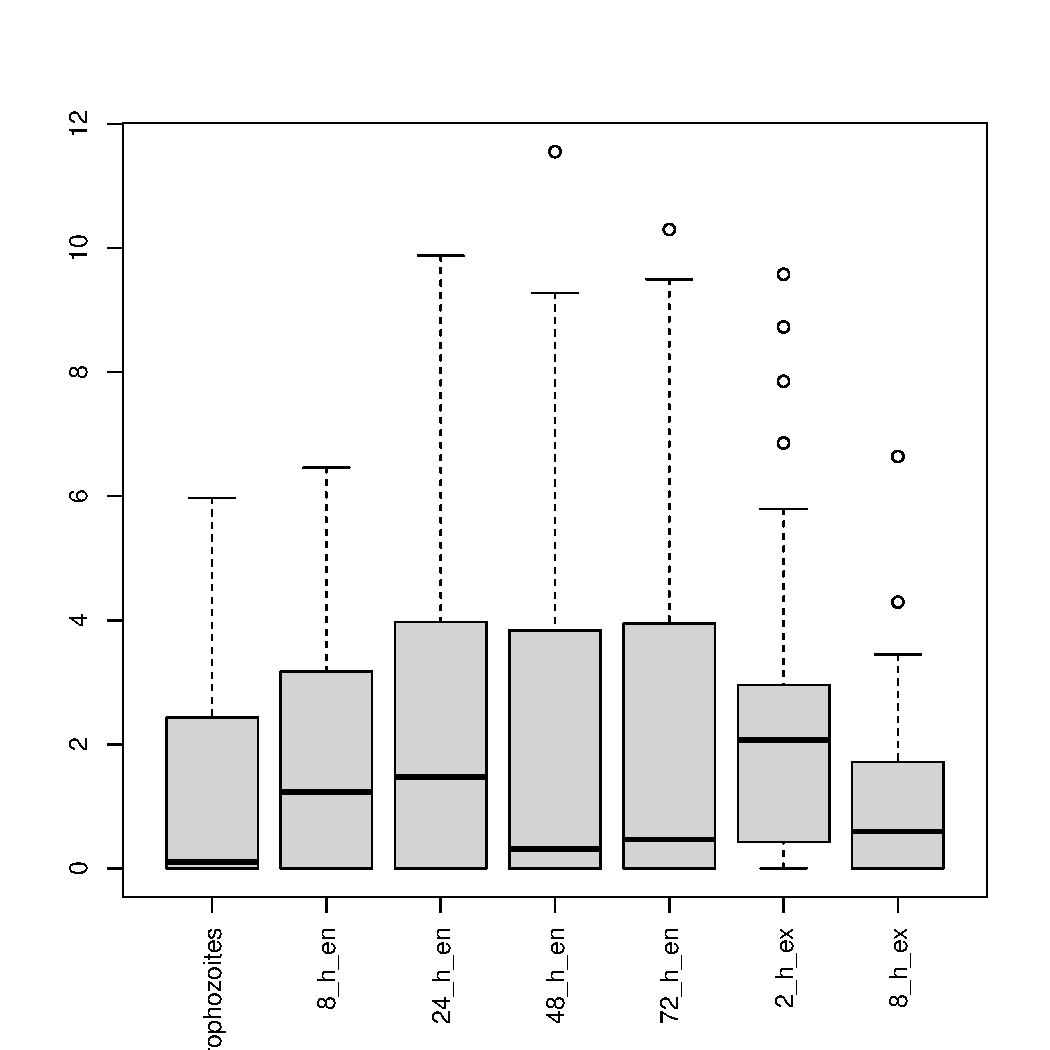
\includegraphics[width=0.8\textwidth]{BoxPlotDatosTransformadosLog2.pdf}
  \caption{Box-plot de los datos despues de aplicarles $Log_{2}$.}
  \label{fig:heatmap_example}
\end{figure}



\end{document}
